\documentclass{article}

\usepackage{latexsym}
\usepackage{fancyhdr}
\usepackage{algorithm}
\usepackage[noend]{algpseudocode}
\usepackage{amsmath}
\usepackage{amsthm}
\usepackage{amssymb}
\usepackage{mathtools}
\usepackage{amsthm}
\usepackage{hyperref}
\usepackage{listings}
\usepackage{scrextend}
\usepackage{dirtytalk}
% \usepackage[demo]{graphicx}
\usepackage{caption}
\usepackage{subcaption}
\usepackage{pdfpages}
\usepackage[shortlabels]{enumitem}
\usepackage[margin=1.2in]{geometry}
\lhead{Charles Pehlivanian}
\rhead{Consecutive Partitions For Power Score Functions}
\cfoot{\thepage}
\pagestyle{fancy}

\hypersetup{colorlinks=true, urlcolor=blue}

\newtheorem{thm}{Theorem}
\newtheorem{definition}{Definition}
\newtheorem{lemma}{Lemma}
\newtheorem{sublemma}{Lemma}[lemma]
\newtheorem{corollary}{Corollary}
\newtheorem{prop}{Proposition}

\newtheoremstyle{case}{}{}{}{}{}{:}{ }{}
\theoremstyle{case}
\newtheorem{case}{Case}

\DeclareMathOperator*{\argmax}{argmax} % thin space, limits underneath in displays
\DeclareMathOperator*{\argmin}{argmin} % thin space, limits underneath in displays
\newcommand{\stirlingii}{\genfrac{\{}{\}}{0pt}{}}

\newenvironment{example}[1]{\par\noindent\underline{Example:}\space#1}{}

\newenvironment{claim}[1]{\par\noindent\underline{Claim:}\space#1}{}
\newenvironment{claimproof}[1]{\par\noindent\underline{Proof:}\space#1}{\hfill $\blacksquare$}

\makeatletter
\def\BState{\State\hskip-\ALG@thistlm}
\makeatother

\begin{document}
\sloppy

\begin{abstract}
	A number of combinatorial optimization problems involve maximization or minimization of the sum of an $\mathbb{R}$-valued set function $F$ over subsets of a partitions of a base set $S$. A common case occurs when the base set is finite $\left\lbrace 1, \dots, n\right\rbrace$, and each element is associated with attributes $x_i$, $y_i$. The inner step of many iterative algorithms - gradient boosting, unsupervized clustering, image compression, network detection - rely on maximization of a power function $F(x,y) = \frac{x^{\gamma}}{y}$ over a suitably labeled base set. It is well-known that the maximization problem for submodular $F$ is NP-hard. We give a set of conditions on $F$ so that exact results can be obtained by constrained maximization over a much smaller set of partitions, for any attribute labeling. We also fill a gap in the existing literature by clearly distinguishing strict and weak size $T$ partitions. The results allow for $\mathcal{O}\left( n^{T-1}\right)$ maximization, although it is shown that with unbounded memory the problem is no worse than $\mathcal{O}\left(n^2\right)$. Finally many of the linear time subset scan algorithms (LTSS) in a spatial scan statistics setting can be obtained with this approach.
\end{abstract}

\section{Preliminaries}
Throughout $n \in \mathbb{N}$ is positive and $N = \{1, \dots, n\}$. Let $X = \left\lbrace x_1, \dots, x_n\right\rbrace$, $Y = \left\lbrace y_1, \dots, y_n\right\rbrace$ be real sequences with $y_i > 0$, for all $i$. The tuple $\left(x_i, y_i\right)$ is called a $\textit{record}$ and denoted by $R_i$. Denote by $\mathcal{D} = \mathcal{D}_{X,Y}$ the set of records associated with the sequences $X$, $Y$. The pairing $R_i = \left(x_i, y_i\right)$ is rigid, but the ordering of the records is exogenously determined by a priority function. 

\begin{definition}
A priority function is a function $G\colon \mathbb{R} \times \mathbb{R}^{+} \to \mathbb{R}$ that induces a total ordering on the tuples $R_i = \left(x_i, y_i\right)$. We refer to $G(x,y) = \frac{x^{\tau}}{y}$ as a power priority function, and the case $\tau = 1$ as the standard priority function. The ordering induced on the sequences $X$, $Y$ induced by $G$ is denoted by $R_{(1)}, R_{(2)}, \dots R_{(n)}$, representing, in order, the highest priority record, next highest, etc., with $X_{\left( i\right)}$, $Y_{\left( i\right)}$ the components of the record $R_{\left( i\right)}$.
\end{definition}

No continuity or smoothness assumpations are made on $G$ for the time being. A partition $\mathcal{P}$ of size $T$ of $N$ is specified by a set of subsets $\mathcal{P} = \{ \pi_1, \dots, \pi_T \}$, $\pi_i \subseteq N$, $i = 1, \dots, T$, such that $P_1 \cup \dots \cup P_T = \{1, \dots, n\}$, with the $P_i$'s pairwise disjoint. Each subset $\pi \in \mathcal{P}$ can be identified with a point $p_\pi = (\sum_{i \in \pi} x_i, \sum_{i \in \pi}y_i) \in \mathbb{R}^2$, with $P_{\emptyset} = (0,0)$ by convention. In this way $\mathcal{P}$ is associated with a pointset in $\mathbb{R}^2$.

The elements $x_i$ and $y_i$ can be thought of as contributing to a scalar score for the record $R_i$. Often $x_i$ is a realization or exceedence and $y_i$ is a baseline expectation. This is the approach taken in online spatial event detection methods in the context of spatial scan statitistics, for detection of disease outbreak, illicit/terrorist activity, and many related surveillance problems. Concentrated subregions of unusual activity are isolated by maximizing a spatial scan statistic. In the parametric case the spatial scan statisitic is a maximum likelihood ratio statistic giving rise to a score for each location, identified by the index $i$. The parametric assumption determines the score function, and maximal score subsets of locations are determined by scanning over the $2^N$ subset locations. Occurence from Gaussian, Poisson processes are common assumptions, giving rise to quadratic and logarithmic score functions, respectively. For many classes of functions - quasiconvex, convex - the search is amenable to an exact linear-time algorithm, $\textit{Linear Time Subset Scanning}$ $(\cite{article6})\textsl{•}$. We give an alternative geometric derivation of the main $LTSS$ result. Alternatively, in a hypothesis testing framework, the parameter space can be divided into regions for which the null is accepted or rejected, with $x_i$ corresponding to the probability of a Type I error, $y_i$ to a Type II error, and the Neyman-Pearson lemma describes an maximal partition for the linear score function $\frac{x_i}{y_i}$. We formalize the notion of a score function on the set $\mathcal{D}$.


\begin{definition}
A score function is a continuous $F(x, y)\colon \mathbb{R} \times \mathbb{R}^{+} \to \mathbb{R}$, strictly increasing in $x$ and strictly decreasing in $y$, with $F\left( 0,0\right) = 0$. If F is of the form $F(x,y) = \frac{x^\gamma}{y}$ for some $\gamma > 0$, then F is a power score function. 
\end{definition}

Several additional properties have been associated with score functions, namely quasi-convexity, componentwise convexity, or a marginal contribution constraint $\frac{x}{y} \frac{\partial F}{\partial x} + \frac{\partial F}{\partial y} \geq 0$ related to submodularity. In particular we do not assume smoothness beyond continuity, nor (quasi)convexity, unless explicitly stated.

A score function $F$ gives rise to a function (also denoted by $F$ when the context is clear) $F \colon 2^N \rightarrow \mathbb{R}$ by summation over individual subset elements $F(S) = F(\sum_{i \in S} x_i, \sum_{i \in S} y_i)$, for $S \subseteq N$. Associating $S \subseteq N$ with its $X$, $Y$ atrributes as in $S = \left\lbrace \left(x_i, y_i\right) \colon i \in S\right\rbrace$, with $X_S = \left\lbrace x_i \colon \left( x_i, y_i\right) \in S\right\rbrace$, $Y_S = \left\lbrace y_i \colon \left( x_i, y_i\right) \in S\right\rbrace$ allows us to write $F(S) = F(X_S, Y_S) = F(\sum_{x \in X_S}x, \sum_{y \in Y_S}y)$, etc.

Now fix a partition $\mathcal{P} = \left\lbrace \pi_1, \dots, \pi_T\right\rbrace$ of size $T$ of $N$. We are interested in maximal partitions for $F$, i.e., solutions to the program
\begin{align} \label{eq0}
\mathcal{P}^{*} = \argmax_{\substack{\mathcal{P} = \left\lbrace \pi_1 \dots, \pi_T\right\rbrace}} {\sum\limits_{j=1}^{T}F\left( X_j, Y_j\right)} = \argmax_{\substack{\mathcal{P} = \left\lbrace \pi_1, \dots, \pi_T\right\rbrace}} {\sum\limits_{j=1}^{T}F( \sum_{i \in \pi_j}x_i, \sum_{i \in \pi_j}y_i)}
\end{align}
which for a power score function becomes
\begin{align} \label{eq1}
\mathcal{P} = \argmax_{\substack{\mathcal{P} = \left\lbrace \pi_1 \dots, \pi_T\right\rbrace}}\sum_{j=1}^{T}\frac{(\sum_{i \in \pi_j}x_i)^\gamma}{\sum_{i \in \pi_j}y_i}
\end{align}

\vspace{4pt}

For example, given a set of quadratic polynomials $f_i(x) = \frac{1}{2}h_ix^2 + g_ix + c_i$, with $h_i >0$ for all $i$, the $x$ values of the vertices are given by $\frac{-g_i}{h_i}$, with minimum values $\frac{-g_i^2}{2h_i}$. The standard priorty function puts an ordering on the vertices sequences $\left\lbrace g_i\right\rbrace$, $\left\lbrace h_i  \right\rbrace$ which is equivalent to projection onto the x-coordinate of the vertex $\left(\frac{-g_i}{h_i},\frac{-g_i^2}{2h_i}\right)$. For $T = 1$, we can easily minimize the sum $\sum_{i=1}^{n} f_i(x)$. For $T >= 2$ the optimization in $\ref{eq1}$ with $\gamma = 2$ finds the $x$-values $\left\lbrace x_1, \dots x_T\right\rbrace$ and the partition that minimize the sum $\sum_{j=1}^T \sum_{i \in P_j} f_i\left( x_j\right)$. This can also be viewed in the context of splittings in each iteration of a gradient boosting algorithm, in which the maximal partition represents the optimal leaf values for a classifier that can take at most $T$ distinct values.

It is well-known that for $F$ submodular, the maximization program above is NP-hard (while the minimization problem can be solved in polynomial time) $\cite{article7}$. A complete search of the space of size $T$ partitions is only feasible for small $N$, say $N \leq 20$, see below It will be necessary to constrain our attention to a smaller set of partitions.

\begin{definition}
A subset $S \subseteq N$ is consecutive if it is of the form $\left\lbrace j, j+1, \dots k\right\rbrace$, for $1 \leq j \leq k \leq n$, or it is the empty set. A consecutive subset $\pi \subseteq N$ is nonsplitting if both $\pi$, $N  \backslash \pi$ are consecutive. Otherwise, it is splitting. Define
\begin{align*}
\mathcal{C} &= \mathcal{C}_N = \{ \pi \subseteq N : \pi \textrm{ is consecutive} \}\\
\mathcal{U} &= \mathcal{U}_N = \{ \pi \subseteq N : \pi \textrm{ is consecutive, non-splitting}\} \\
\mathcal{S} &= \mathcal{S}_N = \mathcal{C} \backslash \mathcal{U} = \{ \pi \subseteq N : \pi \textrm{ is consecutive, splitting} \}
\end{align*}
\end{definition}

A special case of a consecutive subset occurs when $\pi$ is a singleton $\left\lbrace j\right\rbrace$; the pair $\pi$, $N\setminus \pi$ will be called a $\textit{singleton}$ splitting or non splitting pair, depending on whether $N\setminus \pi$ is consecutive. The set of singleton splitting subsets is deonted by $\underline{\mathcal{S}} = \underline{\mathcal{S}}_N \subseteq \mathcal{S}_N$. It is easy to see that $| \mathcal{U_N} | = 2n - 1$, $| \mathcal{S_N} | = \frac{(n-1)(n-2)}{2}$, with $|\mathcal{C_N}| = |\mathcal{U_N}| + |\mathcal{S_N}| = \frac{n(n+1)}{2}$. Therefore, a search over consecutive non-splitting subsets can be performed in linear time, and over consecutive splitting subsets in quadratic time.

\begin{definition}
A partition $\mathcal{P} = \left\lbrace \pi_1, \dots, \pi_T\right\rbrace$ of $N$ of size $T$ such that each $\pi_i$ is an consecutive subset is called a consecutive partition. If every subset of a consecutive partition is nonempty, then it is strongly consecutive, otherwise we allow a weakly consecutive partition to contain $S < T$ nonempty subsets.
\end{definition}

It is known (see $\cite{article1}$, $\cite{article2}$) that if $F$ is convex in all of its arguments, and $y > 0$, that a weakly consecutive partition exists that is maximal in the sense of $\ref{1}$ for the standard priority function. The authors allude to the possibility of empty partition subsets (weakly consecutive partition) as a kind of degenerate case that falls out of the regular line of reasoning. Unfortunately, even in the convex case we can only assure that the maximal partition has size $S \leq T$, and degeneracy is tied to a common occurence in a polytope associated with the sequences $X$, $Y$ (see below). Furthermore, the collapsing of size can be dramatic.

\vspace{4pt}

\begin{example}
Let $X = \left\lbrace 8, 2, 9\right\rbrace$, $Y = \left\lbrace  8, 1, 3\right\rbrace$, $G$ the standard priority function and $F$ the power score function with $\gamma = 4$. It is clear that $F$ is componentwise convex and convex. There are 3 partitions of the set $N = \left\lbrace 1,2,3 \right\rbrace$ and direct evaluation gives
\begin{verbatim}
      PARTITION: [[1, 2], [3]]
          SUBSET: [1, 2] SUBSET SCORE: 1111.1111
          SUBSET: [3] SUBSET SCORE: 2187.0
          PARTITION SCORE: 3298.1111
      PARTITION: [[1], [2, 3]]
          SUBSET: [1] SUBSET_SCORE: 512.0
          SUBSET: [2, 3] SUBSET SCORE: 3660.25
          PARTITION SCORE: 4172.25
      PARTITION: [[1, 3], [2]]
          SUBSET: [1, 3] SUBSET SCORE: 7592.8182
          SUBSET: [2] SUBSET SCORE: 16.0
          PARTITION SCORE: 7608.8182
      MAX PARTITION SCORE: 7608.8182, MAX_PARTITION: [[1, 3], [2]]
\end{verbatim}
In this case no strongly consecutive partition of size 2 exists as the optimal partition is nonconsecutive. A weakly consecutive partition of size $T = 1$ exists consisiting of the trivial partition of $N$ with maximal score
\begin{verbatim}
      PARTITION: [[1, 2, 3]]
          SUBSET: [1, 2, 3] SUBSET SCORE: 10860.0833
          PARTITION SCORE: 10860.0833
      MAX PARTITION SCORE: 10860.0833, MAX_PARTITION: [[0, 1, 2]].
\end{verbatim}  
\end{example}

\begin{example}
Let 
\begin{align*}
X & = \left\lbrace 0.992819, 0.04904, 0.622353, 0.464107, 0.608956, 0.984192 \right\rbrace \\
Y & = \left\lbrace 0.935323, 0.02541, 0.279373, 0.205452, 0.24599, 0.315633 \right\rbrace,
\end{align*}
$G$ the standard priority and $\gamma = 4$. $\frac{X}{Y} \approx \left\lbrace 1.0614718, 1.9299488, 2.2276777, 2.2589559, 2.4755315, 3.118153 \right\rbrace$. $F$ is again convex, but the only maximal consecutive partition of weak size $T = 5$ is the trival size-1 partition. We have

\begin{verbatim}
    Maximal 5-partition
    PARTITION: [ 0 5 ][ 1 ][ 2 ][ 3 ][ 4 ]
    SUM OF SCORES: 13.5342629367

    Maximal 4-partition
    PARTITION: [ 0 4 5 ][ 1 ][ 2 ][ 3 ]
    SUM OF SCORES: 30.6365105858

    Maximal 3-partition
    PARTITION: [ 0 2 4 5 ][ 1 ][ 3 ]
    SUM OF SCORES: 59.8732051128

    Maximal 2-partition
    PARTITION: [ 0 2 3 4 5 ][ 1 ]
    SUM OF SCORES: 91.7825870559

    Maximal 1-partition
    PARTITION: [ 0 1 2 3 4 5 ]
    SUM OF SCORES: 95.5586821397
\end{verbatim}
In fact the trivial partition is the optimal partition of size $T \leq 5$, and there are no strongly consecutive maximal partitions for any $T \in \left\lbrace 2, 3, 4, 5\right\rbrace$.

\end{example}
In fact for any pair $\left( N, T\right)$ a maximally-degenerate collapsing exists for any score function that isn't componentwise subadditive. The guarantee of a weakly consecutive maximizing partition does not constrain the domain of $\cite{eq1}$ nor does it help reduce running time of the optimization. In particular, any search over the consecutive partitions of size $T$ at the top level is incomplete; it may be the case that the optimal partition is weakly consecutive, which says nothing about the optimizing partition of strict size $T$. A complete search of the space must be performed unless the existence of a strongly consecutive partition is guaranteed. If one is looking for the maximal consecutive partition in the first place, one must optimize over all consecutive partitions of size $1, \dots, T$. Thus there is no efficiency gain if one knows in advance only that the optimal partition is weakly consecutive. 

\vspace{4pt}

It will be shown that, for a power priority and score function, the guaranteed existence of a strongly consecutive maximal partition is rare. $\ref{thm0}$. An improved, efficient determination of the optimal partition, whether weak or strict size $T$ is described, allowing for a search over a smaller subset and a worst-case $O(N^2)$ algorithm $\textit{even in the weakly consecutive case}$. Applications are given in Section 3.

\section{Main Results}
We now state our main results. 

\begin{definition}
For any $\mathcal{P}$ a partition of $N$, the partition polytope $\mathcal{C} \subseteq \mathbb{R}^2$ of $\mathcal{P}$ is defined by $\mathcal{C} = convhull \left( \left\lbrace p_\pi : \pi \in \mathcal{P}\right\rbrace \right)$. The constrained partition polytope of $\mathcal{P}$ is defined by $\underline{\mathcal{C}} = convhull \left( \left\lbrace p_\pi : \pi \in \mathcal{P}, \pi \neq \emptyset , \pi \neq N\right\rbrace \right)$
\end{definition}

With a priority function $G$ specified, a subset of records in $\mathcal{D}$ is consecutive if it is of the type $\left\lbrace R_{(j)}, R_{(j+1)}, \dots, R_{(k)}\right\rbrace$, for $1 \leq j \leq k \leq n$ with the ordering from $G$. For the following Proposition, the importance of the standard priority function is established.

\begin{prop} \label{prop0}
Let $\mathcal{D}$ be a set of records with standard priorty function $G$. Let $\mathcal{P}$ be a partition of $N$, and define $\mathcal{E} = \mathcal{E}_\mathcal{C} = \left\lbrace \textit{extreme points of } \mathcal{C}\right\rbrace$, $\underline{\mathcal{E}} = \mathcal{E}_{\underline{\mathcal{C}}} = \left\lbrace \textit{extreme points of } \underline{\mathcal{C}}\right\rbrace$. Then
\begin{enumerate}[(i)]
	\item $\mathcal{E} = \{p_\pi$ : $\pi \in \mathcal{U}_N$\}
	\item $\underline{\mathcal{E}} \supseteq \left\lbrace p_{\pi} \colon \pi \in \mathcal{U}_N \setminus \left\lbrace p_{\emptyset}, p_N \right\rbrace \right\rbrace$, and denoting the right-hand set by $P_{\underline{\mathcal{U}_N}}$ we have 
	\item $\underline{\mathcal{E}} \setminus P_{\underline{\mathcal{U}_N}} \subseteq \left\lbrace p_{\pi} \colon \pi \in \underline{\mathcal{S}_N} \right\rbrace$
\end{enumerate}
In particular $\underline{\mathcal{E}}$ may contain splitting elements, but only associated with singleton splitting paris, while $\mathcal{E}$ contains only nonsplitting elements.
\end{prop}
\begin{proof}
Let $p ^* = (x^*, y^*) \in \mathcal{E}$. Then there is an affine $a\left(x,y\right) = Ax + By + C$ satisfying $a(x^*, y^*) = 0$, $a(x,y) < 0$ for all $(x,y) \in \mathcal{C} \setminus p^*$.  We have
\begin{align}
Ax^* + By^* = \min_{(x,y) \in \mathcal{C}} Ax + By = \min_{\pi \subseteq N} \sum_{i \in \pi} (Ax_i + By_i).
\end{align}
The set $S^* = \{ i \in N: Ax_i + By_i \leq 0 \}$ minimizes the last expression. We will show that $S^*, N\setminus S^*$ are both consecutive. If $A = 0$ then necessarily $B \neq 0$. If $B > 0$ then $S^* =\left\lbrace i \in N \colon y_i \leq 0 \right\rbrace = \emptyset$, otherwise $S^* = \left\lbrace i \in N \colon y_i \geq 0 \right\rbrace$ = N, in either case both $S^*$, $N\setminus S^*$ are consecutive. If $ A \neq 0$ then $S^* = \left\lbrace i \in N \colon \frac{x_i}{y_i} \leq \frac{-B}{A} \right\rbrace$ or $S^* = \left\lbrace i \in N \colon \frac{x_i}{y_i} \geq \frac{-B}{A} \right\rbrace$, depending on the sign of $A$, as $y_i > 0$ for all $i$. In either case, $S^*, N\setminus S^*$ are both consecutive. So $\mathcal{E} \subseteq \mathcal{U}_N$.

Now let $p \in \left\lbrace p_{\pi} \colon \pi \in \mathcal{U}_N\right\rbrace$. Then $\pi = \left\lbrace j.j+1, \dots, k \right\rbrace$, for some $1 \leq j \leq k \leq n$, with either $j = 1$ or $k = n$, or both. Consider first the $j = 1$ case.

\begin{case} $j = 1$, $1 \leq k < n$

Here $p = \left( \sum_{i=1}^k x_i, \sum_{i=1}^k y_i\right)$. For $0 \leq i \leq n+1$ define $C_x^i = \sum_{j=1}^i x_j$, $C_y^i = \sum_{j=1}^i y_j$, $C_x^{-i} = \sum_{j=i}^n x_j$, $C_y^{-i} = \sum_{j=i}^n y_j$, with the convention $C_x^0 = C_y^0 = C_x^{-(n+1)} = C_y^{-(n+1)} = 0$, and $x_0 = y_0 = 0$, so that we can write, for $0  \leq k,l \leq n+1$
\[   
C_x^l - C_x^k = \left\{
\begin{array}{ll}
  \hphantom{-}0, & l = k, \\
  \hphantom{-}\sum_{k+1}^l x_i, & l > k, \\
  -\sum_{l+1}^k x_i, & l < k, \\
\end{array} 
\right. 
\]
\[   
C_x^{-l} - C_x^{-k} = \left\{
\begin{array}{ll}
  \hphantom{-}0, & l = k, \\
  -\sum_k^{l-1} x_i, & l > k, \\
  \hphantom{-}\sum_l^{k-1} x_i, & l < k, \\
\end{array} 
\right. 
\],
with analagous results holding for $C_y^l$, $C_y^{-l}$. Define the affine transformations, for $1 \leq k \leq n-1$
\begin{align*}
l_k^1 &= \left( -y_k, x_k\right) \cdot \left( x,y\right) - \left( -y_kC_x^{k-1} + x_kC_y^{k-1}\right) \\
l_k^2 &= \left( -y_{k+1}, x_{k+1}\right) \cdot \left( x,y\right) - \left( -y_{k+1}C_x^k + x_{k+1}C_y^k\right),
\end{align*}
Note that $l_1^1 = \left( -y_1, x_1\right) \cdot \left( x,y\right)$. Furthermore $l_k^1$ is identically zero on the segment from $\left( C_x^{k-1}, C_y^{k-1}\right)$ to $\left( C_x^k, C_y^k\right)$, and $l_k^2$ is identically zero on the segment from $\left( C_x^k, C_y^k\right)$ to $\left( C_x^{k+1}, C_y^{k+1}\right)$. We will show that $l_k^1 < 0$, $l_k^2 < 0$ on $\mathcal{C}$ outside of the 2 segments above so that $p$ being the intersection of two 1-dimensional facets, is a vertex and extreme point of $\mathcal{C}$. By the first part of the proof, it is sufficient to show that the transformations are negative on points in $\mathcal{U}_N \supseteq \mathcal{E}$ outside of the set  $V = \left\lbrace \left( C_x^{k-1}, C_y^{k-1}\right), \left( C_x^k, C_y^k\right), \left( C_x^{k+1}, C_y^{k+1}\right)\right\rbrace$, as negativity on the interior follows. Write $p = \left( C_x^k, C_y^k\right)$, and consider the transformations $l_k^1, l_k^2$ at points $\left( C_x^l, C_y^l\right)$ or $\left( C_x^{-l}, C_y^{-l}\right)$, for $1 \leq l \leq n$, $l \not \in  \left\lbrace k-1, k, k+1\right\rbrace$. These points are of the form $\left( C_x^l, C_y^l\right)$ or $\left( C_x^{-l}, C_y^{-l}\right)$.

\begin{lemma}
For $\frac{x_1}{y_1} \leq \frac{x_2}{y_2} \leq \dots \leq \frac{x_k}{y_k}$, $y_i > 0$, for all $i$,
\begin{align*}
\frac{x_1}{y_1} \leq \frac{x_1 + \dots + x_k}{y_1 + \dots + y_k} \leq \frac{x_k}{y_k},
\end{align*}
with equality if and only if $\frac{x_1}{y_1} = \dots = \frac{x_n}{y_n}$.
\end{lemma}
\begin{proof}
The proof is by induction on $k$. For $k=2$, using the fact that $x_2y_1 - x_1y_2 \geq 0$, we have
\begin{align*}
\frac{x_1+x_2}{y_1+y_2} - \frac{x_1}{y_1} = \frac{x_1y_2 - x_2y_1}{y_1\left( y_1 + y_2\right)} &\geq 0 \\
\frac{x_1 + x_2}{y_1 + y_2} - \frac{x_2}{y_2} = \frac{x_1y_2 - x_2y_1}{y_2\left( y_1 + y_2\right)} &\leq 0.
\end{align*}
For $k > 2$, two applications of the above case gives
\[
\frac{x_1}{y_1} \leq \frac{\sum_1^{k-1} x_i}{\sum_1^{k-1} y_i} \leq \frac{\sum_1^k x_k}{\sum_1^k y_i} \leq \frac{x_k}{y_k}. 
\]
If $\frac{x_1}{y_1} = \frac{x_n}{y_n}$, then the ordering in the assumptions implies all ratios are equal. 
\end{proof}

Thus for $k+1 < l < n$,
\begin{align*}
l_k^1\left( C_x^l, C_y^l\right) &= -y_kC_x^l + x_kC_y^l + y_kC_x^{k-1} - x_kC_y^{k-1} \\
&= \left( \frac{x_k}{y_k} - \frac{\sum_k^l x_i}{\sum_k^l y_i}\right)y_k\left( \sum_k^l y_i\right) \\
&< 0
\end{align*}
and
\begin{align*}
l_k^2\left(C_x^l, C_y^l\right) &= -y_{k+1}C_x^l + x_{k+1}C_y^l + y_{k+1}C_x^k - x_{k+1}C_y^k \\
&= \left( \frac{x_{k+1}}{y_{k+1}} - \frac{\sum_{k+1}^l x_i}{\sum_{k+1}^l y_i}\right)y_{k+1}\left( \sum_{k+1}^l y_i\right) \\
&< 0
\end{align*}
Similarly, for $1 \leq l < k-1$,
\begin{align*}
l_k^1\left( C_x^l, C_y^l\right) &= \left( \frac{\sum_{l+1}^{k-1} x_i}{\sum_{l+1}^{k-1} y_i} - \frac{x_k}{y_k}\right)y_k\left( \sum_{l+1}^{k-1} y_i\right) \\
&\leq \left( \frac{\sum_{l+1}^{k-1} x_i}{\sum_{l+1}^{k-1} y_i} - \frac{x_{k-1}}{y_{k-1}}\right)y_k\left( \sum_{l+1}^{k-1} y_i\right) \\
&< 0
\end{align*}
and 
\begin{align*}
l_k^2\left(C_x^l, C_y^l\right) &= \left( \frac{\sum_{l+1}^k x_i}{\sum_{l+1}^k y_i} - \frac{x_{k+1}}{y_{k+1}}\right) y_{k+1}\left(\sum_{l+1}^{k}y_i\right) \\
&\leq \left( \frac{\sum_{l+1}^k x_i}{\sum_{l+1}^k y_i} - \frac{x_k}{y_k}\right) y_{k+1}\left(\sum_{l+1}^{k}y_i\right)\\
&< 0.
\end{align*}
We also have, for $k+1 < l \leq n$,
\begin{align*}
l_k^1\left( C_x^{-l}, C_y^{-l}\right) &= -y_kC_x^{-l} + x_kC_{y}^{-l} + y_kC_x^{k-1} - x_kC_y^{k-1} \\
&= \left( \frac{x_k}{y_k} - \frac{\sum_l^n x_i}{\sum_l^n y_i}\right)y_k \left( \sum_l^n y_i\right) + \left( \frac{\sum_1^{k-1} x_i}{\sum_l^{k-1}y_i} - \frac{x_k}{y_k}\right)y_k \left( \sum_1^{k-1}y_i\right) \\
&< 0
\end{align*}
and
\begin{align*}
l_k^2\left( C_x^{-l}, C_y^{-l}\right) &= -y_{k+1}C_x^{-l} + x_{k+1}C_y^{-l} + y_{k+1}C_x^k - x_{k+1}C_y^k \\
&= \left( \frac{x_{k+1}}{y_{k+1}} - \frac{\sum_l^n x_i}{\sum_l^n y_i}\right)y_{k+1}\left(\sum_l^n y_i\right) + \left( \frac{\sum_1^k x_i}{\sum_1^k y_i} - \frac{x_{k+1}}{y_{k+1}}\right)y_{k+1}\left(\sum_1^k y_i\right) \\
&< 0,
\end{align*}
while for $1 \leq l < k-1$,
\begin{align*}
l_k^1\left( C_x^{-l}, C_y^{-l}\right) &= -y_kC_x^{-l} + x_kC_{y}^{-l} + y_kC_x^{k-1} - x_kC_y^{k-1} \\
&=\left( \frac{x_k}{y_k} - \frac{\sum_k^nx_i}{\sum_k^ny_i}\right)y_k\left(\sum_k^n y_i\right)  + \left( \frac{\sum_1^{l-1}x_i}{\sum_1^{l-1}y_i} - \frac{x_k}{y_k}\right)y_k\left(\sum_1^{l-1}y_i\right) \\
&< 0,
\end{align*}
and
\begin{align*}
l_k^2\left( C_x^{-l}, C_y^{-l}\right) &= -y_{k+1}C_x^{-l} + x_{k+1}C_y^{-l} + y_{k+1}C_x^k - x_{k+1}C_y^k \\
&= \left( \frac{x_k}{y_k} - \frac{\sum_{k+1}^nx_i}{\sum_{k+1}^ny_i}\right)y_k\left( \sum_{k+1}^n y_i\right) + \left( \frac{\sum_1^{l-1}x_i}{\sum_1^{l-1}y_i} - \frac{x_k}{y_k}\right)y_k\left( \sum_1^{l-1}y_i\right) \\
&< 0.
\end{align*}
Thus the sets $\left\lbrace \left( x,y\right) \colon l_k^1\left( x,y\right) = 0\right\rbrace$, $\left\lbrace \left( x,y\right) \colon l_k^2\left( x,y\right) = 0\right\rbrace$ define two one-dimensional facets whose intersection $p$ is an extreme point of $\mathcal{C}$.
\end{case}

\begin{case} $j = 1$, $k = n$

In this case $p = \left(C_x^n, C_y^n\right) = \left( C_x^{-1}, C_y^{-1}\right)$. The transformations needed in this case are
\begin{align*}
l_n^1 &= \left( -y_n, x_n\right) \cdot \left( x,y\right) - \left( -y_nC_x^{n-1} + x_nC_y^{n-1}\right) \\
l_n^2 &= \left( y_1, -x_1\right) \cdot \left( x,y\right) - \left( y_1C_x^{-2} - x_1C_y^{-2}\right),
\end{align*}
\end{case}
One can again check that $l_n^1\left( p\right) = -y_nC_x^n + x_nC_y^n + y_nC_x^{n-1} - x_nC_y^{n-1} = 0$, and $l_n^2\left( p\right) = y_1C_x^n - x_1C_y^n - y_1C_x^{-2} + x_1C_y^{-2} = 0$, that $l_n^1$ is identially zero on the segment from $\left( C_x^{n-1}, C_y^{n-1}\right)$ to $\left( C_x^n, C_y^n\right)$ and that $l_n^2$ is identically zero on the segment from $\left( C_x^n, C_y^n\right)$ to $\left( C_x^{-2}, C_y^{-2}\right)$. Furthermore, for any point in $\mathcal{U}_n$ of the form $\left( C_x^l, C_y^l\right)$ for $1 \leq l < n-1$, or $\left( C_x^{-l}, C_y^{-l}\right)$ for $2 < l \leq n$ we show that both transformations are negative.

For a point in $\mathcal{E}$ of the form $\left( C_x^l, C_y^l\right)$, with $1 \leq l < n-1$, we have
\begin{align*}
l_n^1\left( C_x^l, C_y^l\right) &= -y_nC_x^l + x_nC_y^l + y_nC_x^{n-1} - x_nC_y^{n-1} \\
&= \left( \frac{\sum_{l+1}^{n-1}x_i}{\sum_{l+1}^{n-1}y_i} - \frac{x_n}{y_n}\right) y_n\left( \sum_{l+1}^{n-1}y_i\right) \\
&< 0
\end{align*}
and
\begin{align*}
l_n^2\left( C_x^l, C_y^l\right) &= y_1C_x^l - x_1C_y^l - y_1C_x^{-2} + x_1C_y^{-2} \\
&= \left( \frac{x_1}{y_1} - \frac{\sum_{l+1}^n x_i}{\sum_{l+1}^n y_i}\right)y_1\left( \sum_{l+1}^n y_i\right) \\
&< 0
\end{align*}
For a point in $\mathcal{E}$ of the form $\left(C_x^{-l},C_y^{-l}\right)$, with $2 < l \leq n$, we have
\begin{align*}
l_n^1\left( C_x^{-l},C_y^{-l}\right) &= -y_nC_x^{-l} + x_nC_y^{-l} + y_nC_x^{n-1} - x_nC_y^{n-1} \\
&= \left( \frac{\sum_1^{l-1}x_i}{\sum_1^{l-1}y_i} - \frac{x_n}{y_n}\right) y_n\left( \sum_1^{l-1}y_i\right) \\
&< 0
\end{align*}
and
\begin{align*}
l_n^2\left( C_x^{-l},C_y^{-l}\right) &= y_1C_x^{-l} -x_1C_y^{-l} - y_1C_x^{-2} + x_1C_y^{-2} \\
&= \left( \frac{x_1}{y_1} - \frac{\sum_2^{l-1}x_i}{\sum_2^{l-1}y_i}\right)y_1\left( \sum_2^{l-1}y_i\right) \\
&< 0
\end{align*}

So once again p is the intersection of two one-dimensional facets and is an exterme point of $\mathcal{C}$.

\begin{case} $k = n$, $1 < j < n$

In this case $p = \left( C_x^{-j}, C_y^{-j}\right)$ and the vanishing affine transformations are given by
\begin{align*}
l_j^1 &= \left( y_{j+1}, -x_{j+1}\right) \cdot \left( x,y\right) - \left( y_{j+1}C_x^{-j} - x_{j+1}C_y^{-j}\right) \\
l_j^2 &= \left( y_j, -x_j\right) \cdot \left( x,y\right) - \left( y_jC_x^{-\left(j+1\right)} - x_jC_y^{-\left( j+1\right)}\right)
\end{align*}
One can again check that $l_j^1$ is identically zero on the segment from $\left( C_x^{-(j-1)}, C_y^{-(j-1)}\right)$ to $\left( C_x^{-j}, C_y^{-j}\right)$ and that $l_j^2$ is identically zero on the segment from  $\left( C_x^{-j}, C_y^{-j}\right)$ to $\left( C_x^{-(j+1)}, C_y^{-(j+1)}\right)$. It can again be shown that $l_j^1$, $l_j^2$ are strictly negative on the points in $\mathcal{U}_N$ outside of the 3 boundary points of the segments above. The details are technical and analogous to the above calculations. The conclusion that $p$ is an extreme point again follows.
\end{case} 

Thus $\mathcal{U}_N \subseteq \mathcal{E}$, and the proof of part i) is complete.

We now prove that $\underline{\mathcal{E}} \subseteq P_{\underline{\mathcal{P}_N}} \cup P_{\underline{\mathcal{S}_N}}$, where $P_{\mathcal{\underline{P}_N}} = \left\lbrace p_{\pi} \colon \pi \in \mathcal{U}_N \setminus \left\lbrace p_{\emptyset}, p_N \right\rbrace \right\rbrace$, $P_{\underline{\mathcal{S}_N}} = \left\lbrace p_{\pi} \colon \pi \in \underline{\mathcal{S}_N} \right\rbrace$. For $\underline{\pi}^* = \left( \underline{x}^*, \underline{y}^* \right) \in \underline{\mathcal{E}}$, we can again find a separating affine function $l\left( x,y\right) = Ax + By + C$, satisfying
\begin{align} \label{eq6}
A\underline{x}^* + B\underline{y}^* =\min_{\substack{S \subseteq N \\ S \neq \emptyset \\ S \neq N}} \sum_{i \in S} \left( Ax_i + By_i\right)
\end{align}
Let $\pi^* = \argmin_{S \in N} \sum_{i \in S} \left( Ax_i + By_i\right)$, which by the previous argument is of the form $\left\lbrace j, j+1, \dots, k\right\rbrace$. If $\vert \pi^* \vert = m$, with $1 < m < n$, then it also minimizes $\ref{eq6}$, is consecutive, non-splitting, and $\pi^* \subseteq \underline{\mathcal{P}_N}$. Otherwise there are 2 cases.

\setcounter{case}{0}
\begin{case} $\pi^* = \emptyset$. 
Since the minimizing set can be written $\pi^* = \left\lbrace i \in N \colon Ax_i + By_i \leq 0 \right\rbrace$, we must have $Ax + By > 0$ for $\left( x,y\right) \in \mathcal{C}$. So $\ref{eq6}$ is minimized by selecting $\underline{\pi}^* = \left\lbrace i^*\right\rbrace$, for $i^* = \argmin_i \left( Ax_i + By_i\right)$, a singleton. $\underline{\pi}^*$ therefore lies in either $P_{\underline{\mathcal{P}_N}}$ or $P_{\underline{\mathcal{S}_N}}$, depending on whether $N \setminus p_{\pi}$ is consecutive.
\end{case}
\begin{case} $\pi^* = N$. Then by similar reasoning, $Ax_i + By_i < 0$ for all $\left( x,y\right) \in \mathcal{C}$. Thus $\ref{eq6}$ is minimized by removing a single element from $N$; take $\underline{\pi}^* = N\setminus \left\lbrace i^*\right\rbrace$, where $i^* = argmax_{i \in N} \left( Ax_i + By_i\right)$. Again $\underline{\pi}^*$ lies in either $P_{\underline{\mathcal{P}_N}}$ or $P_{\underline{\mathcal{S}_N}}$.
\end{case}
So $\underline{\mathcal{E}} \subseteq P_{\mathcal{\underline{P_N}}} \cup P_{\mathcal{S}_N}$. Now let $p = p_{\pi}$ be an element of $P_{\mathcal{\underline{P_N}}}$, so that $\pi \in \mathcal{U}_N \setminus \left\lbrace p_{\emptyset}, p_N\right\rbrace$. From the first part of the proof, to any such $p_{\pi}$ we can associate two affine maps $l_k^1, l_k^2$, where $\pi = \left\lbrace k, k+1, \dots, n\right\rbrace$ or $\pi = \left\lbrace 1, \dots, k-1, k\right\rbrace$, for $1 \leq k \leq n$, such that $l_k^1\left( p_{\pi}\right) = l_k^2\left( p_{\pi}\right) = 0$, and $l_k^1, l_k^2 \vert_{\mathcal{C}} < 0$. Hence $l_k^1, l_k^2 \vert_{\mathcal{\underline{C}}} < 0$, and by definition $P_{\mathcal{\underline{P_N}}} \subseteq \underline{\mathcal{E}}$. This completes the proof of parts ii), iii), and we have completed the classification of extreme points for $\underline{\mathcal{C}}$ as desired.
\end{proof}

\vspace{6pt} 
The vertices of $\mathcal{C}$ can be found by a purely geometric construction, the basis of which is a ``sweeping`` argument that lies at the root of a Graham scan $\cite{article3}$ used to find the vertices of a convex hull of a point set in $\mathbb{R}^2$. Writing $\frac{x_1}{y_1} \leq \dots \frac{x_q}{y_q} \leq 0 \leq \frac{x_{q+1}}{y_{q+1}} \leq \dots \frac{x_n}{y_n}$, we have 
\begin{align} \label{eq7}
\frac{y_q}{x_q} \leq \dots \frac{y_1}{x_1} \leq 0 \leq \frac{y_n}{x_n} \leq \dots \leq \frac{y_{q+1}}{x_{q+1}}.
\end{align} 
In addition, if $y_1, y_2 > 0$, and $x_1$, $x_2$ are of the same sign, then $\frac{y_2}{x_2} \leq \frac{y_1+y_2}{x_1+x_2} \leq \frac{y_1}{x_1}.$ By repeated application it follows that
\begin{align} \label{eq8}
\frac{y_M}{x_M} \leq \frac{\sum_{i \in S}y_i}{\sum_{i \in S}x_i} \leq \frac{y_m}{x_m}
\end{align}
for any $S \subseteq N$, where $m = \min S$, $M = \max S$. 

The construction of the convex hull of $\mathcal{C}$ follows. Since all $y_i > 0$, the point $p_{\emptyset} = \left(0,0\right)$ has the miminal y-coordinate in the set $\mathcal{C}$. Starting with this point (necessarily in the set of vertices of $\mathcal{C}$), and sweeping a ray from the negative x-axis in a clockwise direction $\pi$ radians to the positive x-axis, it follows that the first point of the form $p_{\left\lbrace i \colon i \in N\right\rbrace}$ encountered during the sweep is $p_{\left\lbrace 1 \right\rbrace}$, from $\ref{eq7}$. In fact the points $p_{\left\lbrace i \right\rbrace}$, $i =1, \dots q$ will be met in order during the sweep, although most (all except 2) are not vertices of $\mathcal{C}$. From the relation $\frac{y_2}{x_2} \leq \frac{y_1+y_2}{x_1+x_2} \leq \frac{y_1}{x_2}$ it follows that the segment from point $p_{\left\lbrace 1,2 \right\rbrace}$ to the origin subtends an angle (with the negative x axis) that is between that formed by $p_{\left\lbrace 1 \right\rbrace}$ and $p_{\left\lbrace 2 \right\rbrace}$, although its y-coordinate is larger than both. We can also place the point $p_{\left\lbrace 2,3 \right\rbrace}$ in this way, it subtends a smaller angle (as measured from the negative x-axis) than $p_{\left\lbrace 1,2 \right\rbrace}$. From the relation $\frac{y_2+y_3}{x_2+x_3} \leq \frac{y_1+y_2+y_3}{x_1+x_2+x_3} \leq \frac{y_1}{x_1}$, the angle formed by the segment joining $p_{\left\lbrace 1, 2, 3\right\rbrace}$ lies between that formed by $p_{1}$ and the origin, and $p_{2,3}$ and the origin. Building the convex hull in this way we can see that $p_{2,3}$ is "shadowed" by the points $p_{1,2}$, $p_{1,2,3}$ and is in the interior, not part of the vertices of $\mathcal{C}$. The argument can be generalized to show that $\mathcal{C}$ - $\left\lbrace p_{\left\lbrace 1\right\rbrace}, p_{\left\lbrace 1,2 \right\rbrace}, \dots, p_{\left\lbrace 1, \dots, n\right\rbrace}, p_{\left\lbrace 2, \dots, n\right\rbrace}, p_{\left\lbrace 3, \dots, n\right\rbrace}, \dots, p_{\left\lbrace n\right\rbrace}\right\rbrace = \left\lbrace p_{\pi} \colon \pi \in \mathcal{U}_N\right\rbrace$. See Figures 1, 2.

The process to determine the vertices of the convex hull of $\underline{\mathcal{C}}$ is similar. From $\ref{prop0}$, all points determined above are obtained as vertices, in order, with the exception of $p_{\emptyset} = \left( 0,0\right)$, $p_N = \left( \sum_{1}^n x_i, \sum_{1}^n y_i\right)$. After removing these, the additional splitting singleton pairs are considered as some or all may be vertices. Since these pairs are indexed by $1 < i < n$, they can be listed and tested successively. If any one is a vertex, it will lie between $p_{\left\lbrace n\right\rbrace}$ and $p_{\left\lbrace 1\right\rbrace}$ when the vertices of $\mathcal{C}$ are traversed in a clockwise direction. If any lies below the segment joining these two vertices, then there is a splitting pair in $\underline{\mathcal{E}}$. If more than one does, we can use the familiar right-turn rule to determine which of these are vertices: for $p^1$, $p^2$, $p^3$ with increasing x-coordinates, $p^2$ is in the lower convex hull if and only if
\[
\begin{vmatrix} \label{eq8}
p_x^1 & p_y^1 & 1\\
p_x^2 & p_y^2 & 1\\
p_x^3 & p_y^3 & 1\\
\end{vmatrix} > 0.
\]
Otherwise $p^2 \in int\left( \underline{\mathcal{C}}\right)$. We can use Algorithm 1 to determine all extreme points for $\underline{\mathcal{C}}$, given a configuration $X$, $Y$.

\begin{algorithm}
\caption{Extreme Point Algorithm for Cosntrained Partition Polytope }
\begin{algorithmic}[1]
\State $\underline{\mathcal{E}} \leftarrow \left\lbrace p_{\pi} \colon \pi \in U_N\right\rbrace$
\State $L \leftarrow \left\lbrace p_{\pi} \colon \pi = \left\lbrace i\right\rbrace, 1 \leq i \leq n\right\rbrace$
\State sort $L$ by decreasing x-coordinate
\State $s[0] \leftarrow \textit{pop}\left( L\right)$, $s[1] \leftarrow \textit{pop}\left( L\right)$
\For{$i = \textit{size}\left( L\right) \textit{step -1}$}
\State $p_i = \textit{pop}\left( L\right)$
\State append $p_i$ to $s$
\State $p^1$, $p^2$, $p^3 \leftarrow$ last 3 points of $s$
\If{$\begin{vmatrix}
p_x^1 & p_y^1 & 1\\
p_x^2 & p_y^2 & 1\\
p_x^3 & p_y^3 & 1\\
\end{vmatrix} > 0.$}
\State remove middle of last 3 points from $s$
\EndIf
\EndFor
\State $S \leftarrow S \cup \left\lbrace N\setminus \pi \colon \pi \in S\right\rbrace$
\State $\underline{\mathcal{E}} \leftarrow \underline{\mathcal{E}} \cup S$\
\end{algorithmic}
\end{algorithm}

Now introduce a symmetric score function $\overline{F}\colon \mathcal{C} \subseteq \mathbb{R} \times \mathbb{R}^{+} \to \mathbb{R}$ by
\[   
\overline{F}\left( x,y\right) = \left\{
\begin{array}{ll}
      F\left( x,y\right) + F\left( C_x-x, C_y-y\right), & \left( x,y\right) \in \Omega \setminus{\left\lbrace \left( 0,0\right), \left( C_x, C_y\right) \right\rbrace}  \\
      F\left( x,y\right), & \left( x,y\right) \in \left\lbrace \left( 0,0\right), \left( C_x, C_y\right) \right\rbrace  \\
\end{array} 
\right. 
\]
where $C_x = \sum_1^n x_i$, $C_y = \sum_1^n y_i$. $\overline{F}$ is continuous on $\Omega \subseteq \mathbb{R} \times \mathbb{R}^{+}$ for any score function $F$. In addition the convexity/concavity, and componentwise convexity/concavity of $\overline{F}$ on its domain is inherited from the corresponding properties of $F$, although submodularity, subadditivity, quasiconvexity are not.

\vspace{16pt}
\begin{figure}
\centering
\begin{subfigure}{.5\textwidth}
  \centering
  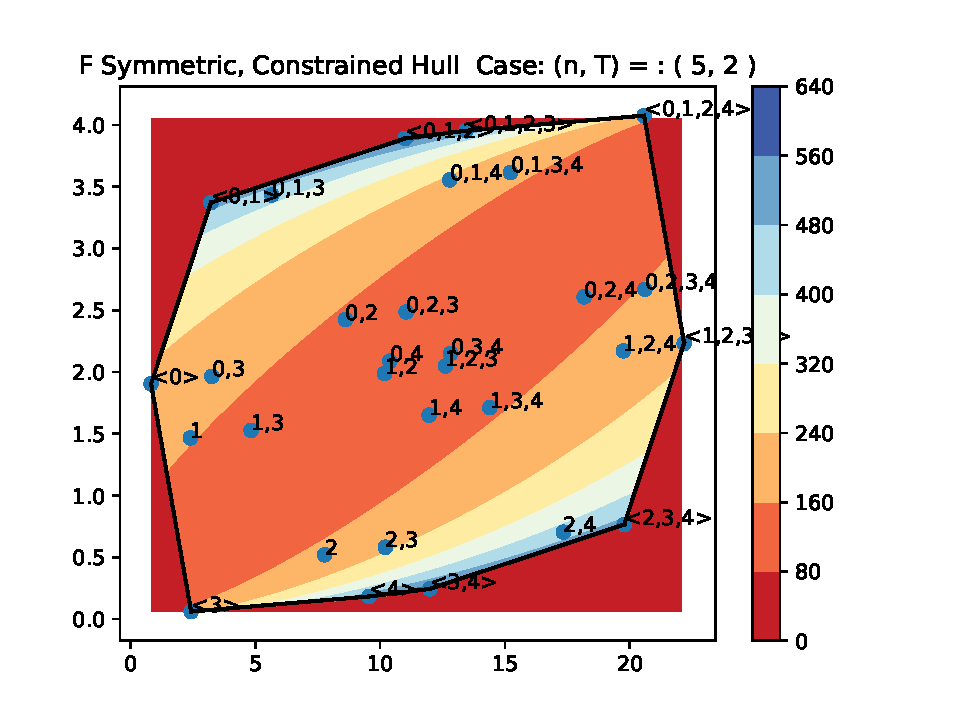
\includegraphics[scale=.55]{const_hull_5_2.pdf}
  \caption{(n,T) = (5,2)}
  \label{fig:sub1}
\end{subfigure}%
\begin{subfigure}{.5\textwidth}
  \centering
  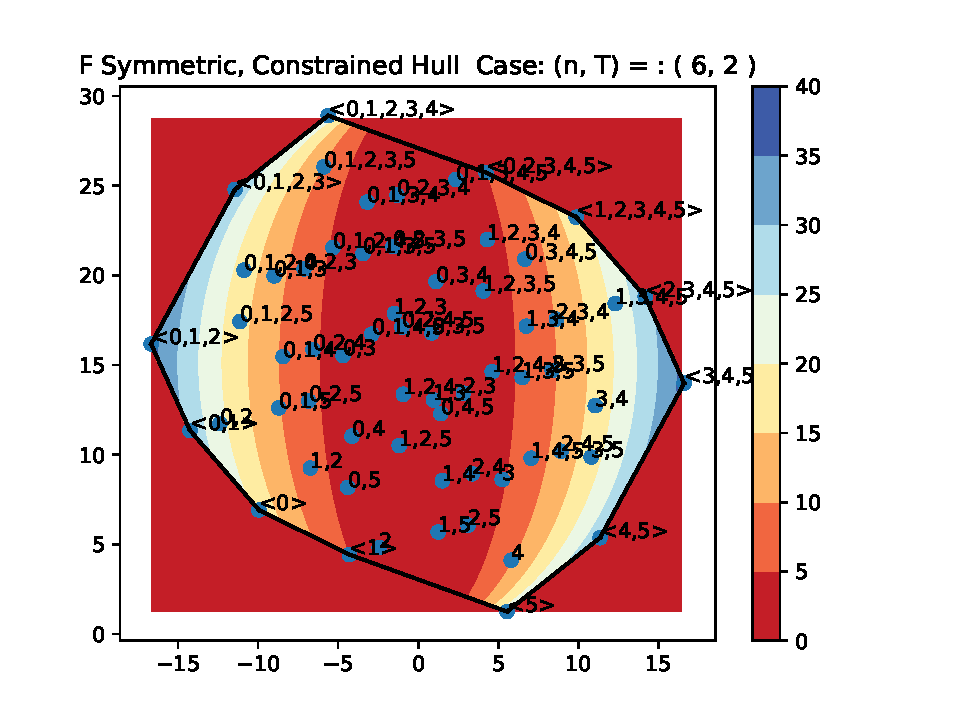
\includegraphics[scale=.55]{const_hull_6_2.pdf}
  \caption{(n,T) = (6,2)}
  \label{fig:sub2}
\end{subfigure}
\caption{Constrained convex hull $\underline{\mathcal{C}}$ for (n,T) = (5,2), (6,2) $N = \left\lbrace 0,1, \dots, n-1 \right\rbrace$ with level sets for the symmetric $\overline{F}$ with $\gamma = 2$. Vertices are labeled by $<>$, and the consecutive splitting partition pair associated with $\left\lbrace 3\right\rbrace$, $\left\lbrace 0, 1, 2, 4\right\rbrace$ lie on the hull in (a), while the the consecutive splitting pair $\left\lbrace 1\right\rbrace$, $\left\lbrace 0, 2, 3, 4, 5\right\rbrace$ lie on the hull in (b).}
\label{fig:hull1}
\end{figure}

\vspace{6pt}
\begin{figure}
\centering
\begin{subfigure}{.5\textwidth}
  \centering
  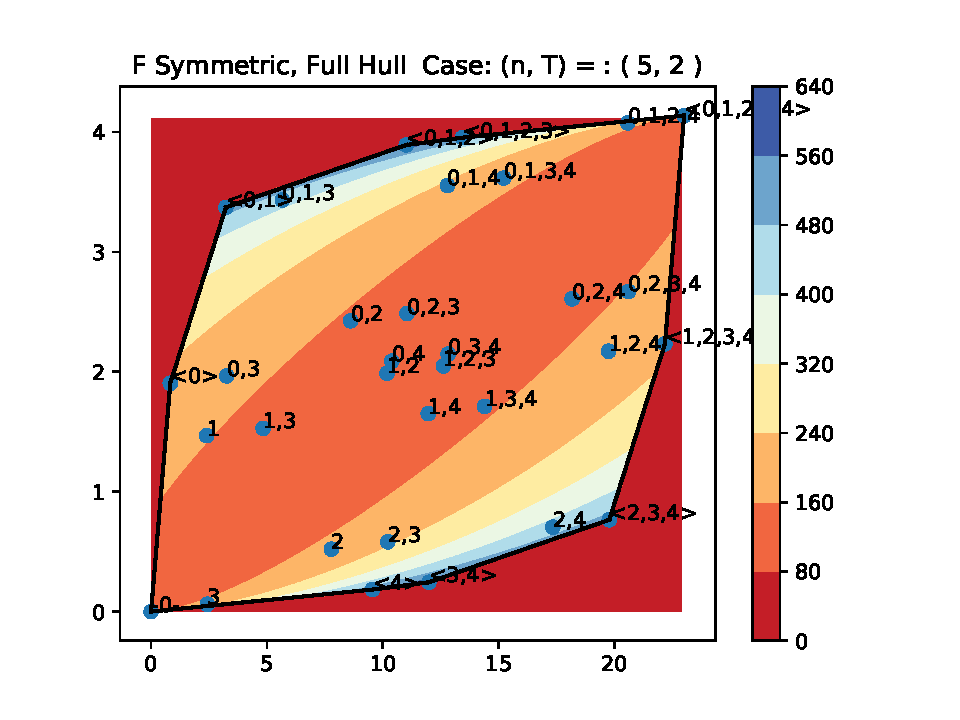
\includegraphics[scale=.55]{full_hull_5_2.pdf}
  \caption{(n,T) = (5,2)}
  \label{fig:sub1}
\end{subfigure}%
\begin{subfigure}{.5\textwidth}
  \centering
  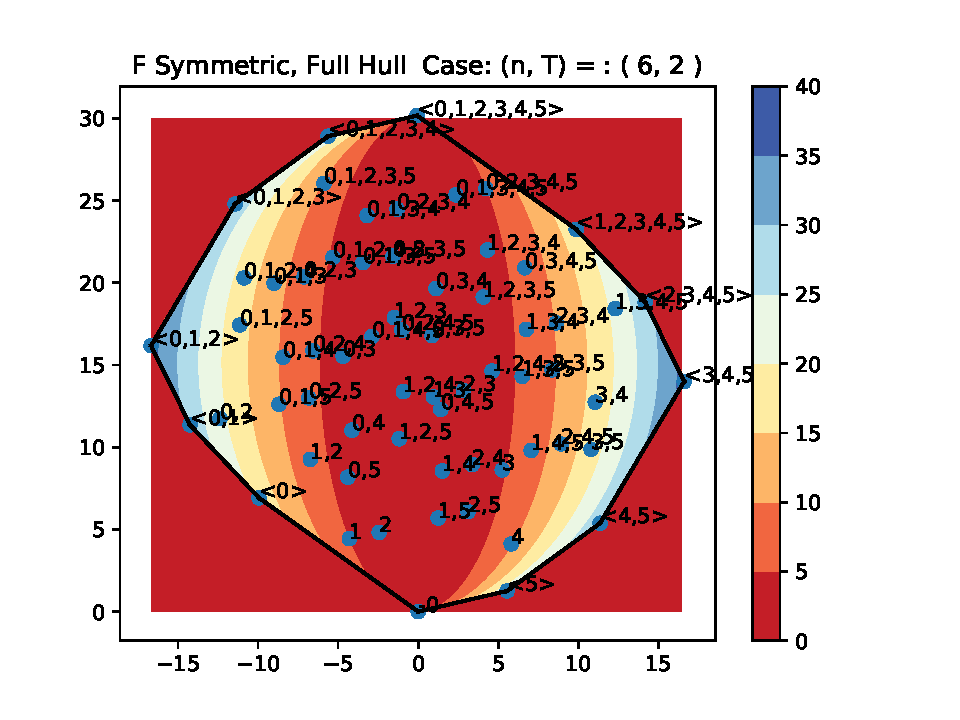
\includegraphics[scale=.55]{full_hull_6_2.pdf}
  \caption{(n,T) = (6,2)}
  \label{fig:sub2}
\end{subfigure}
\caption{Full convex hull for the above cases, only consecutive non-splitting partition points lie on both hulls.}
\label{fig:test}
\end{figure}

\begin{prop}
Let $F$ be quasiconvex, or convex in each of its arguments. If $\argmax_{\left( x,y\right) \in \underline{\mathcal{C}}} \overline{F}\left( x,y\right) \in \mathcal{S}_N$, then $p_N = \argmax_{\left( x,y\right) \in \mathcal{C}} \overline{F}$, and all of the $x_i$ are of the same sign.
\end{prop}
\begin{proof}
Let $\underline{p} = \argmax_{\left( x,y\right) \in \underline{\mathcal{C}}} \overline{F}\left( x,y\right)$, with $\underline{p}$ consecutive splitting in $N$. Let $p = \argmax_{\left( x,y,\right) \in \mathcal{C}} \overline{F}\left( x,y\right)$. The elementwise convexity or quasiconvexity of $\overline{F}$ on $\mathcal{C}$, $\hat{p} \in \mathcal{E}$ follows from the corresponding property of $F$, so $p \in \mathcal{E}$. Since $\underline{\mathcal{C}} \subseteq \mathcal{C}$, $\overline{F}\left( p\right) \geq \overline{F}\left( \underline{p}\textsl{•}\right)$. Since $\underline{p}$ is not an extreme point of $\mathcal{C}$ by the previous proposition, we have $\overline{F}\left( p\right) > \overline{F}\left( \underline{p}\right)$, so $p$ cannot lie in $\underline{\mathcal{E}}$. The only elements in $\mathcal{E}\setminus \underline{\mathcal{E}}$ are $\left\lbrace p_{\emptyset}, p_{N}\right\rbrace$, and since $\overline{F}\left( p_{\emptyset}\right) = \overline{F}\left( p_N\right)$, the first part follows. Finally, if $\overline{F}$ is maximaixed at $p_N$ and there is a $1 \leq q < n$ with $\frac{x_1}{y_1} \leq \dots \leq \frac{x_q}{y_q} \leq 0 \leq \frac{x_{q+1}}{y_{q+1}} \leq \dots \leq \frac{x_n}{y_n}$, then by strict monotonicity of $F$ in $x$, $y$, we have $F\left( \sum_{q+1}^n x_i, \sum_{q+1}^n y_i\right) > F\left( p_N\right)$, hence $\overline{F}\left( \sum_{q+1}^n x_i, \sum_{q+1}^n y_i\right) > F\left( p_N\right) = \overline{F}\left( p_N\right)$, unless $q = 0$ or $q = n$, in which case all of the $x_i$ of the same sign.
\end{proof}

The existence of maximal consecutive partitions will be invesigated for fixed priority, score functions, and arbitrary $X$, positive $Y$. In the case of power score functions their existence is rare (Theorem $\ref{thm0}$ below), unless we constrain $X$. For the unconstrained case the desired property is property (S) of $F$, $G$
\vspace{8pt}

\begin{addmargin}[2em]{2em} \label{propA}
\begin{list}{(Property S)}{}
\item For given $F$, $G$ score and priority functions, any $n$ and any $T < n$, the solution to $\ref{eq1}$ is achieved at a strongly consecutive partition, for any $X \subseteq \mathbb{R}$, $Y \subseteq \mathbb{R}^+$
\end{list}
\end{addmargin}
\vspace{8pt}
We will also consider existence of a weakly consecutive partition
\vspace{8pt}
\begin{addmargin}[2em]{2em} \label{propA}
\begin{list}{(Property W)}{}
\item For given $F$, $G$ score and priority functions, any $n$ and any $T < n$, the solution to $\ref{eq1}$ is achieved at a weakly consecutive partition, for any $X \subseteq \mathbb{R}$, $Y \subseteq \mathbb{R}^+$
\end{list}
\end{addmargin}
\vspace{8pt}

\begin{thm} \label{thm0}
Let the dataset $\mathcal{D} = \{ \mathbf{R}_1, \ldots, \mathbf{R}_n \}$ be ordered with the standard priority function. Let $F$ be a power score function $F(R_i) = F(x_i,y_i) = \frac{x_i^\gamma}{y_i}$. Then $F$, $G$ have Property S if and only if $\gamma = 2$.
\end{thm}

The set of partitions is greatly reduced by the requirement that $\mathcal{P}$ be consecutive. The set of all partitions of $n$ is the Bell number of order $T$, exponentially increasing with $n$ for any $T > 1$. The set of all size $T$ partitions is a Stirling number of the second kind $\stirlingii{n}{T}$. The $n$th Bell number $B_n$ is given by the identity
\[B_n = \sum_{k=0}^{n} \binom{n}{k} B_k\]
The Stirling numbers follow the recursion
\[S_{n+1,k} = \stirlingii{n+1}{k} = k\stirlingii{n}{k} + \stirlingii{n}{k-1}\]
and have asymptotic growth rate 
\[\stirlingii{n}{k} \sim \frac{k^n}{k!}\]
Let $\mathcal{O}_{n,T}$ be the set of consecutive partitions of $N$ of size $T$. The set of consecutive partitions of $N$ of size $T$ has size $\binom{n-1}{T-1}$, which grows as $\mathcal{O}\left( n^{T-1}\right)$. So for $\left(n,T\right) = \left(20, 10\right)$, we have $\vert S_{n,T}\vert \approx 5.9e12$, $\vert \mathcal{O}_{n,T}\vert = 92378$, while for $\left(n,T\right) = \left(30, 10\right)$, we have $\vert S_{n,T}\vert \approx 1.73e22$, $\vert \mathcal{O}_{n,T}\vert = 10,015,005$.  Although the polynomial growth of $O_{n,T}$ may not be acceptable, especially for large $T$, we outline a dynamic programming approach which guarantees worst-case quadratic time, for any $T$, at the expense of a possibly large memory footprint, as we will see.

\begin{proof}
Let $\left( \gamma, \tau\right) = \left( 2,1\right)$. The proof proceeds by induction on $T$. For $T=2$ define $\overline{F}$ as above. $\ref{eq1}$ then becomes $M = \max_{\left( x,y\right) \in \underline{\mathcal{C}}} \overline{F}\left( x,y,\right)$, which is solved at $p_{\pi}$, for $\pi$, $N\setminus \pi$ consecutive subsets of $N$, unless 
\begin{align} \label{eq8}
p_N = argmax_{\left( x,y\right) \in \mathcal{C}} \overline{F}\left( x,y\right)
\end{align} by Proposition 1. But for any $x_i, y_i \in \mathbb{R}$, $y_i > 0$, $i = 1,2$, we have
\begin{align*}
\left( \sqrt{\frac{y_2}{y_1}}x_1 - \sqrt{\frac{y_1}{y_2}x_2}\right)^2 \geq 0 &\implies \left( x_1+x_2\right)^2 \leq x_1^2\left( \frac{y_1+y_2}{y_1}\right) + x_2^2\left( \frac{y_1+y_2}{y_2}\right)\\
&\implies \frac{\left( x_1+x_2\right)^2}{y_1+y_2} \leq \frac{x_1^2}{y_1} + \frac{x_2^2}{y_2},
\end{align*}
so that for $\gamma = 2$, $F$ satisifies a subadditive property in both variables. In particular, $p_N$ cannot maximize $\ref{eq8}$ above ($\overline{F}$ is in fact $\textit{minimized}$ there), and the solution is a strongly consecutive partition $\pi$, $N\setminus \pi$. 

Now let $T >= 3$. The arguments here a are duplicated from $\cite{article2}$. Define, for any subset $\pi \subseteq N$, $M_{\pi} = \max S$, $m_{\pi} = \min S$, and $d\left(\pi\right) = M_{\pi} - m_{\pi}$. Let $\mathcal{P} = \left\lbrace \pi_1, \dots, \pi_T\right\rbrace$ be a maximal size $T$ partition that maximizes $\ref{eq1}$ which also minimizes $\sum_{j=1}^T d\left(\pi_j\right)$ among all optimal size $T$ partitions. If not all $\pi_j$ are consecutive, then we can find $\pi_i$, $\pi_j$ and $k \in \pi_j$ with $m_{\pi_i} < k < M_{\pi_i}$. Note that $\min\left( M_{\pi_i}, M_{\pi_j}\right) \geq k$,  and $\max\left( m_{\pi_i}, m_{\pi_j} \right) \leq k$, so that 
\[
\min\left( M_{\pi_i}, M_{\pi_j}\right) - \max\left( m_{\pi_i}, m_{\pi_j} \right) \geq 0.
\] 
From proof of the $T = 2$ case, we can find an optimal partition of $\pi_i \cup \pi_j$ into nonempty consecutive sets $\pi^{\prime}_i, \pi^{\prime}_j$ with respect to $\pi_i \cup \pi_j$. Then $d\left( \pi^{\prime}_i\right) + d\left( \pi^{\prime}_j\right) \leq \max\left( M_{\pi_i}, M_{\pi_j}\right) - \min\left( m_{\pi_i}, m_{\pi_j}\right) - 1$, so
\begin{align*}
d\left(\pi_i\right) + d\left( \pi_j\right) &= M_{\pi_i} - m_{\pi_i} + M_{\pi_j} - m_{\pi_j} \\
&= \max\left(M_{\pi_i}, M_{\pi_j}\right) + \min\left(M_{\pi_i}, M_{\pi_j}\right) \\
&- \min\left( m_{\pi_i}, m_{\pi_j} \right) - \max\left( m_{\pi_i}, m_{\pi_j} \right) \\
&\geq d\left(\pi^{\prime}_i\right) + d\left(\pi^{\prime}_j\right) + 1,
\end{align*}
a contradiction. So all of the $\pi_j$ are consecutive, nonempty.

For the necessity choose $\gamma = 2 + \epsilon$, for $\epsilon > 0$. Set
\[
X = \left[ 1-\delta, \delta, 1 + \delta\right], Y = \left[ 1, \delta, 1\right]
\] 
for some $\delta > 0$. There are 3 partitions of $\left\lbrace 1, 2, 3\right\rbrace$, namely $\mathcal{P}_1 = \left\lbrace \left[ 0 \right], \left[ 1, 2\right]\right\rbrace$, $\mathcal{P}_2 = \left\lbrace \left[ 0, 1 \right], \left[ 2\right]\right\rbrace$, and $\mathcal{P}_3 = \left\lbrace \left[ 0, 2 \right], \left[ 1 \right]\right\rbrace$. Only the first 2 are ordered. The scores can be computed
\begin{align*}
\text{Score}\left(\mathcal{P}_1\right) & = \left( 1-\delta \right)^\gamma + \frac{\left( 1+2\delta\right)^\gamma}{1+\delta} \\
\text{Score}\left(\mathcal{P}_2\right) & = \frac{1}{1+\delta} + \left( 1+\delta\right)^\gamma \\
\text{Score}\left(\mathcal{P}_3\right) & = 2^{1+\epsilon}
\end{align*}
The last expression is independent of $\delta$, so can choose $\delta$ small so that the last score dominates.
For $\gamma = 2 - \epsilon$, $\epsilon > 0$, and the sequences
\[
X = \left[ 1, \frac{1}{\delta}, 1\right], Y = \left[ \frac{1}{1+\delta}, \frac{1}{\delta}, \frac{1}{1-\delta}\right]
\] 
we have
\begin{align*}
\text{Score}\left(\mathcal{P}_1\right) & = \frac{1^\gamma}{\frac{1}{1+\delta}} + \frac{\left(1 + \frac{1}{\delta}\right)^\gamma}{\left( \frac{1}{\delta} + \frac{1}{1 - \delta}\right) }  = \frac{\left(1 + \frac{1}{\delta}\right)^\gamma}{\left( \frac{1}{\delta} + \frac{1}{1 - \delta}\right) } + \left( 1 + \delta \right)\\
\text{Score}\left(\mathcal{P}_2\right) & = \frac{1^\gamma}{\frac{1}{1-\delta}} + \frac{\left( 1 + \frac{1}{\delta}\right)^\gamma}{\left( \frac{1}{1+\delta} + \frac{1}{\delta}\right)}  = \frac{\left( 1 + \frac{1}{\delta}\right)^\gamma}{\left( \frac{1}{1+\delta} + \frac{1}{\delta}\right)} + \left( 1 - \delta \right)\\
\text{Score}\left(\mathcal{P}_3\right) & = \frac{\left( 1 + 1\right)^\gamma}{\left(\frac{1}{1+\delta} + \frac{1}{1-\delta}\right)}  + \frac{\left( \frac{1}{\delta}\right)^\gamma}{\frac{1}{\delta}} = \frac{\left( \frac{1}{\delta}\right)^\gamma}{\frac{1}{\delta}} + 2^{\gamma - 1}\left( 1 - \delta^2\right) 
\end{align*}
and letting $\delta \rightarrow 0$ gives the result, as the first summands in each score can be made arbitrarily close to each other.

To extend these examples to larger $\vert \mathcal{D} \vert = M > N$, $S \geq T$, simply add $M-N$ identical records of the form $R_i = \left( 0, y\right)$, for any $y > 0$. Index the new elements by $N+1, \dots, M$. Since $S \geq T$, an unordered candidate partition is formed by adjoining to $\mathcal{P}^{\prime} = \left[\left[0, 2\right], \left[ 1\right]\right]$ an arbitrary partition $\mathcal{P}^{\prime\prime}$ of size $S - T$ of the indices $N+1, \dots, M$, the new partition is $\mathcal{P} = \mathcal{P}^{\prime} \cup \mathcal{P}^{\prime\prime}$. We have $\text{Score}\left(\mathcal{P}\right) = \text{Score}\left(\mathcal{P}^{\prime}\right)$. It is clear that inserting any record in any subset of $\mathcal{P}^{\prime\prime}$ into any subset from a partition in $\mathcal{P}^{\prime}$ only decreases the total score, while inserting a record from $\mathcal{P}^{\prime}$ into $\mathcal{P}^{\prime\prime}$ also represents a decrease from one of the above partitions scores for $\mathcal{P}_1$, $\mathcal{P}_2$, if the element of index 1 is switched, nonetheless the new partition won't be ordered. Of the elements 0, 2, the only one that can be switched while retaining an ordered partition is 2, in which case the new partition is of the form $\left[ \left[ 0\right], \left[ 1\right], \left[ 2, \dots\right]\right]$. But the score of any such partition must be less than
\[
\left( 1-\delta\right)^\gamma + \frac{\delta^\gamma}{\delta} + \left( 1+\delta\right)^\gamma
\]
which is dominated by the unordered partition $\mathcal{P}_3 = \left\lbrace \left[ 0, 2 \right], \left[ 1 \right]\right\rbrace$ above. The argument for $\gamma < 2$ is similar. In this way we can generate optimal, unordered partitions for any $\gamma > 0$ and $\left( N, T\right)$. Therefore $\gamma = 2$.
\end{proof}

Note that for $\gamma = 2$ and priority function $G\left( x,y\right) = \frac{x^{\tau}}{y}$, $\tau = 1$ is the only priority power that guarantees Property S is satisfied. To see this let
\[
X = \left[ x-\delta, \delta, x + \delta\right], Y = \left[ x, \delta, x\right]
\] 
for $x, \delta > 0$, and consider the three partitions $\mathcal{P}_i$, $i=1, 2, 3$ as above. We have
\begin{align*}
& \text{Score}\left(\mathcal{P}_1\right) = \text{Score}\left(\mathcal{P}_2\right) \\
& \text{Score}\left(\mathcal{P}_3\right) - \text{Score}\left(\mathcal{P}_1\right) = \text{Score}\left(\mathcal{P}_3\right) - \text{Score}\left(\mathcal{P}_2\right) = \frac{-\delta^2\left( 2x + \delta\right)}{x\left( x + \delta\right)}
\end{align*}
The power priority $G(x,y) = \frac{x^\tau}{y}$ places the priorty on the records:
\begin{align} \label{eq8}
\left( G(x_1, y_1), G(x_2, y_2), G(x_3, y_3)\right) = \left( \frac{\left( x - \delta \right)^{\tau}}{x}, \delta^{\tau-1},  \frac{\left( x + \delta \right)^{\tau}}{x}\right).
\end{align}
For $\tau > 1$, choosing $x$ large relative to delta gives $G(x_2, y_2) < G(x_1, y_1) < G(x_3, y_3)$. So the partitions $\mathcal{P}_1 = \left\lbrace \left[ 0 \right], \left[ 1, 2\right]\right\rbrace$, $\mathcal{P}_2 = \left\lbrace \left[ 0, 1 \right], \left[ 2\right]\right\rbrace$, and $\mathcal{P}_3 = \left\lbrace \left[ 0, 2 \right], \left[ 1 \right]\right\rbrace$ become $\mathcal{P}_1 = \left\lbrace \left[ 1 \right], \left[ 0, 2\right]\right\rbrace$, $\mathcal{P}_2 = \left\lbrace \left[ 0, 1 \right], \left[ 2\right]\right\rbrace$, and $\mathcal{P}_3 = \left\lbrace \left[ 1, 2 \right], \left[ 0 \right]\right\rbrace$, maintaining the partition scores above. The maximum score is shared by $\mathcal{P}_1$, $\mathcal{P}_2$, the first being unordered. In order to force $\text{Score}\left(\mathcal{P}_1\right) > \text{Score}\left(\mathcal{P}_2\right)$, we perturb the original $X$, $Y$ by
\[
X\left(\epsilon\right) = \left[ x-\delta+\epsilon, \delta, x + \delta\right], Y = \left[ x, \delta, x\right]
\]
and denoting by $\text{Score}\left(\epsilon \right)\left(\mathcal{P}_i \right)$ the score of the partition $\mathcal{P}_i$ on the records $\left\lbrace \left(x\left(\epsilon\right)_1, y_1\right),\left(x\left(\epsilon\right)_2, y_2\right),\left(x\left(\epsilon\right)_3, y_3\right) \right\rbrace$, it follows that
\begin{align*}
\text{Score}\left(\epsilon \right)\left(\mathcal{P}_1 \right) - \text{Score}\left(\mathcal{P}_1 \right) &= \frac{\left( x + \epsilon - \delta\right)^2}{x} - \frac{\left( x - \delta\right)^2}{x} = \frac{2\epsilon\left( x - \delta\right) + \epsilon^2}{x} \\
\text{Score}\left(\epsilon \right)\left(\mathcal{P}_2 \right) - \text{Score}\left(\mathcal{P}_2 \right) &= \frac{\left( x + \epsilon\right)^2}{x + \delta}  - \frac{x^2}{x+\delta}= \frac{2\epsilon x + \epsilon^2}{x+\delta}
\end{align*}
Choosing, e.g. $x = 1$, $\delta = .25$ gives 
\begin{align*}
\text{Score}\left(\epsilon \right)\left(\mathcal{P}_1 \right) - \text{Score}\left(\mathcal{P}_1 \right) &= \frac{3}{2}\epsilon + \epsilon^2 \\
\text{Score}\left(\epsilon \right)\left(\mathcal{P}_2 \right) - \text{Score}\left(\mathcal{P}_2 \right) &= 2\epsilon + \epsilon^2
\end{align*}
By choosing $epsilon > 0$ small enough, we can ensure that the first term, corresponding to the score of the partition $\left[ \left[ 1\right], \left[ 0, 2\right]\right]$ dominates, while the priority order $G(x_2, y_2) < G(x_1, y_1) < G(x_3, y_3)$ is maintained. The maximal partition in this case is therefore unordered.
For $ 0 \leq \tau < 1$ and the priority function $G(X,Y) = \frac{x^{\tau}}{y}$, choose $x$ large relative to $\delta$ forces the priority ordering $G(x_0, y_0) \leq G(x_2, y_2) \leq G(x_1, y_1)$. So the  highest and second highest records exchange priority ordering, and the partition $\mathcal{P}_1$ stays the same, while $\mathcal{P}_1$ now corresponds to $\left\lbrace \left[ 0, 2\right], \left[ 1\right]\right\rbrace$, $\mathcal{P}_2$ to $\left\lbrace \left[ 0, 1\right], \left[ 2\right]\right\rbrace$, only the last being ordered. Perturbing the original sequences by
\[
X\left(\epsilon\right) = \left[ x-\delta, \delta, x + \delta + \epsilon\right], Y = \left[ x, \delta, x\right]
\]
yields
\begin{align*}
\text{Score}\left(\epsilon \right)\left(\mathcal{P}_1 \right) - \text{Score}\left(\mathcal{P}_2 \right) &= \frac{\left( x + 2\delta + \epsilon\right)^2}{x + \delta}  - \frac{\left( x + 2\delta\right)^2}{x + \delta} = \frac{2\epsilon\left( x + 2\delta\right) + \epsilon^2}{x + \delta} \\
\text{Score}\left(\epsilon \right)\left(\mathcal{P}_2 \right) - \text{Score}\left(\mathcal{P}_1 \right) &= \frac{\left( x + \delta + \epsilon\right)^2}{x} - \frac{\left( x + \delta\right)}{x} = \frac{2\epsilon\left( x + \delta \right) + \epsilon^2}{x} \\
\end{align*}
We choose $\epsilon > 0$ small enough so that the first term dominates, corresponding to the unordered partition. Therefore $\tau = 1$.


Theorem 1 is a special case of the following.

\begin{thm} \label{thm1}
Let $\mathcal{D}$, $F$, $G$ be as above, with $\tau = 1$, and $F$ subadditive. Then there is a maximal strongly consecutive partition for any $X \subseteq \mathbb{R}$, $Y \subseteq \mathbb{R}^+$. 
\end{thm}
\begin{proof}
The proof is exactly the same, only subadditivity is used to assure that $\argmin_{(x,y) \in \underline{\mathcal{C}}} F\left( x,y\right) = \argmin_{(x,y) \in \mathcal{C}} F\left( x,y\right)$.
\end{proof}

Since submodular, positive functions are subadditive, we have the following.

\begin{corollary} \label{cor0}
Let $\mathcal{D}$, $F$, $G$ be as above, with $\tau = 1$, and $F$ submodular, positive. Then there is a maximal strongly consecutive partition.
\end{corollary}

The approach above provide an alternative proof of the Linear Time Subset Scanning (LTSS) property of certain subset statistics for spatial scanning problems, in which case a spatial scan statisitic provides the score function (see $\cite{article6}$). The result provides for linear-time cluster detection in the context of disease outbreak, terrorist attacks, etc.

\begin{corollary} \label{cor1}
[See Theorem 1, $\cite{article6}$] Let $\mathcal{D}$, $F$, $G$ be as above, with $F$ quasiconvex. Then $F$ satisfies the Linear Time Subset Scanning property of $\cite{article6}$, i.e., the solution partition
\[
\mathcal{P_0} = \argmax_{S \subseteq N} F(\sum_{i \in S}x_i, \sum_{i \in S}y_i)
\]
is a consecutive subset of $N$.
\end{corollary}
\begin{proof}
Since $F(\lambda X_1 + \left( 1 - \lambda\right)X_2, \lambda Y_1 + \left( 1 - \lambda\right) Y_2) \leq \max{\left(F(X_1, Y_1), F(X_2, Y_2)\right)}$, for all $X_1, X_2$, $Y_1, Y_2 \in \mathcal{C}$, $\lambda \in \left[ 0,1\right]$, it is easy to show that $F$ attains a maximal value over $\mathcal{C}$ at an extreme point, which is a consecutive partition, by Proposition $\cite{prop0}$.
\end{proof}

XXX

In addition, if $F$ is submodular on $2^N$, the optimal partitions display an interleaving property with varying $T$.
\begin{thm} \label{thm2}
With $D$, $F$, $G$ as above, assume that $F$ is submodular on $2^N$. Then there exist maximal consecutive parititions, for $\mathcal{P}_T = \left\lbrace \pi_1^T, \dots, \pi_T^T\right\rbrace$, satisfying, for all $T$, $1 \leq i \leq T-1$
\begin{align*}
\min{\pi_i^T} &\leq \min{\pi_i^{T-1}} \leq \min{\pi_{i+1}^T} \\
\max{\pi_i^T} &\leq \max{\pi_i^{T-1}} \leq \max{\pi_{i+1}^T} \\
\end{align*}
and $\min{\pi_T^T} \leq \max{\pi_T^T} \leq \max{\pi_{T-1}^{T-1}}$.
\end{thm}
\begin{proof}
adapt arguments from $\cite{article5}$.
\end{proof}

A weaker property is introduced, placing constraints on the set $X$.
\vspace{8pt}

\begin{addmargin}[2em]{2em} \label{propA}
\begin{list}{(B)}{}
\item For given $F$, $G$ score and priority functions, any $n$ and any $T < n$, the solution to $\ref{eq1}$ is achieved at a strongly consecutive partition, for any $X, Y \subseteq \mathbb{R}^+$
\end{list}
\end{addmargin}
\vspace{8pt}

\vspace{16pt}

$\underline{\text{Additional cases - write up}}$
\begin{enumerate}
    \item Property (B) holds for $\gamma = 1$
    \item Property (A) holds for any quasiconvex function if $T = 2$ and $X$ is of mixed-sign
    \item Interleaving property allows us to fix problematic weakly consecutive case, $\gamma = 4$, say, by starting with $S = 2$ and considering interleaving partitions to move from $S, S+1, \dots, T$. If any one of the subsets of the partition at step $S$ contains $X$ values of the same sign, it may result in a non-consecutive split of that subset at the next step, if not, the subsets are interleaving, consecutive.
\end{enumerate}

\section{Implementation}
We address a gap in the current literature concerning the case for which $F$ is not subadditive, but admits a weakly maximal consecutive partition. As shown previously, the arguments in $\cite{article1}, \cite{article2}$ only guarantee the existence of maximal weakly consecutive partitions when the score function $F$ is convex in all variables, or quasiconvex. The weakly consecutive partition may have strict size $S$ for $S < T$, and the collapse of size may be complete, to $S = 1$ as we have seen. Any search would require a complete scan of all partitions at level $T$ to find the optimal score, and if the optimal partition is not consecutive, the search would resume at levels $T-1, ...$. There is no efficiency gain unless we know $\textit{a priori}$ that a strict size $S$ optimal consecutive partition exists, or something about the structure of the optimal partition of strict size $T$. We can relax the supermodularity requirment on $F$, obtaining

\begin{thm} \label{thm3}
Let $\mathcal{D}$, $F$, $G$ be as above, with $\tau = 1$. Suppose that $F$ is convex in all arguments. Then for any $1 \leq T \leq N$, there is a maximal strongly singleton splitting partition.
\end{thm}


The brute-force optimization in $\ref{eq1}$ has cost that grows exponentially with $n$. A constrained optimization over the set of all size $T$ ordered partitions has cost that grows as $\binom{n-1}{T-1}$, i.e., as a polynomail of degree $T-1$. In particular, the $T = 2$ problem grows linearly in $n$. There is an improvement that can be made to this approach.

Consider a graph $\mathcal{G} = \left( V, E\right)$ with vertices denoted by $\left( i, j\right)$, for $i \in \left\lbrace 1, \dots, n\right\rbrace$, $j \in \left\lbrace 1, \dots, T\right\rbrace$. Add a source node $\left( 1, 1\right)$ and a terminal sink node labeled $\left( n+1, T+1\right)$, Add directed edges from node $\left( i,k \right)$ to $\left( i, k+1\right)$, for each $i < j$, with edge cost $\frac{-\left(\sum_{r=i}^{j-1} x_r\right)^2}{\sum_{r=i}^{j-1} y_r}$. The interpretation is that a path from node $\left( i, j\right)$ to $\left( k, j+1\right)$ represents choice of the subset $\left\lbrace i, \dots, k\right\rbrace$ as the $i^{th}$ subset in the candidate partition. One can then solve for the shortest path by finding a shortest path by the Bellman-Ford algorithm. 


% 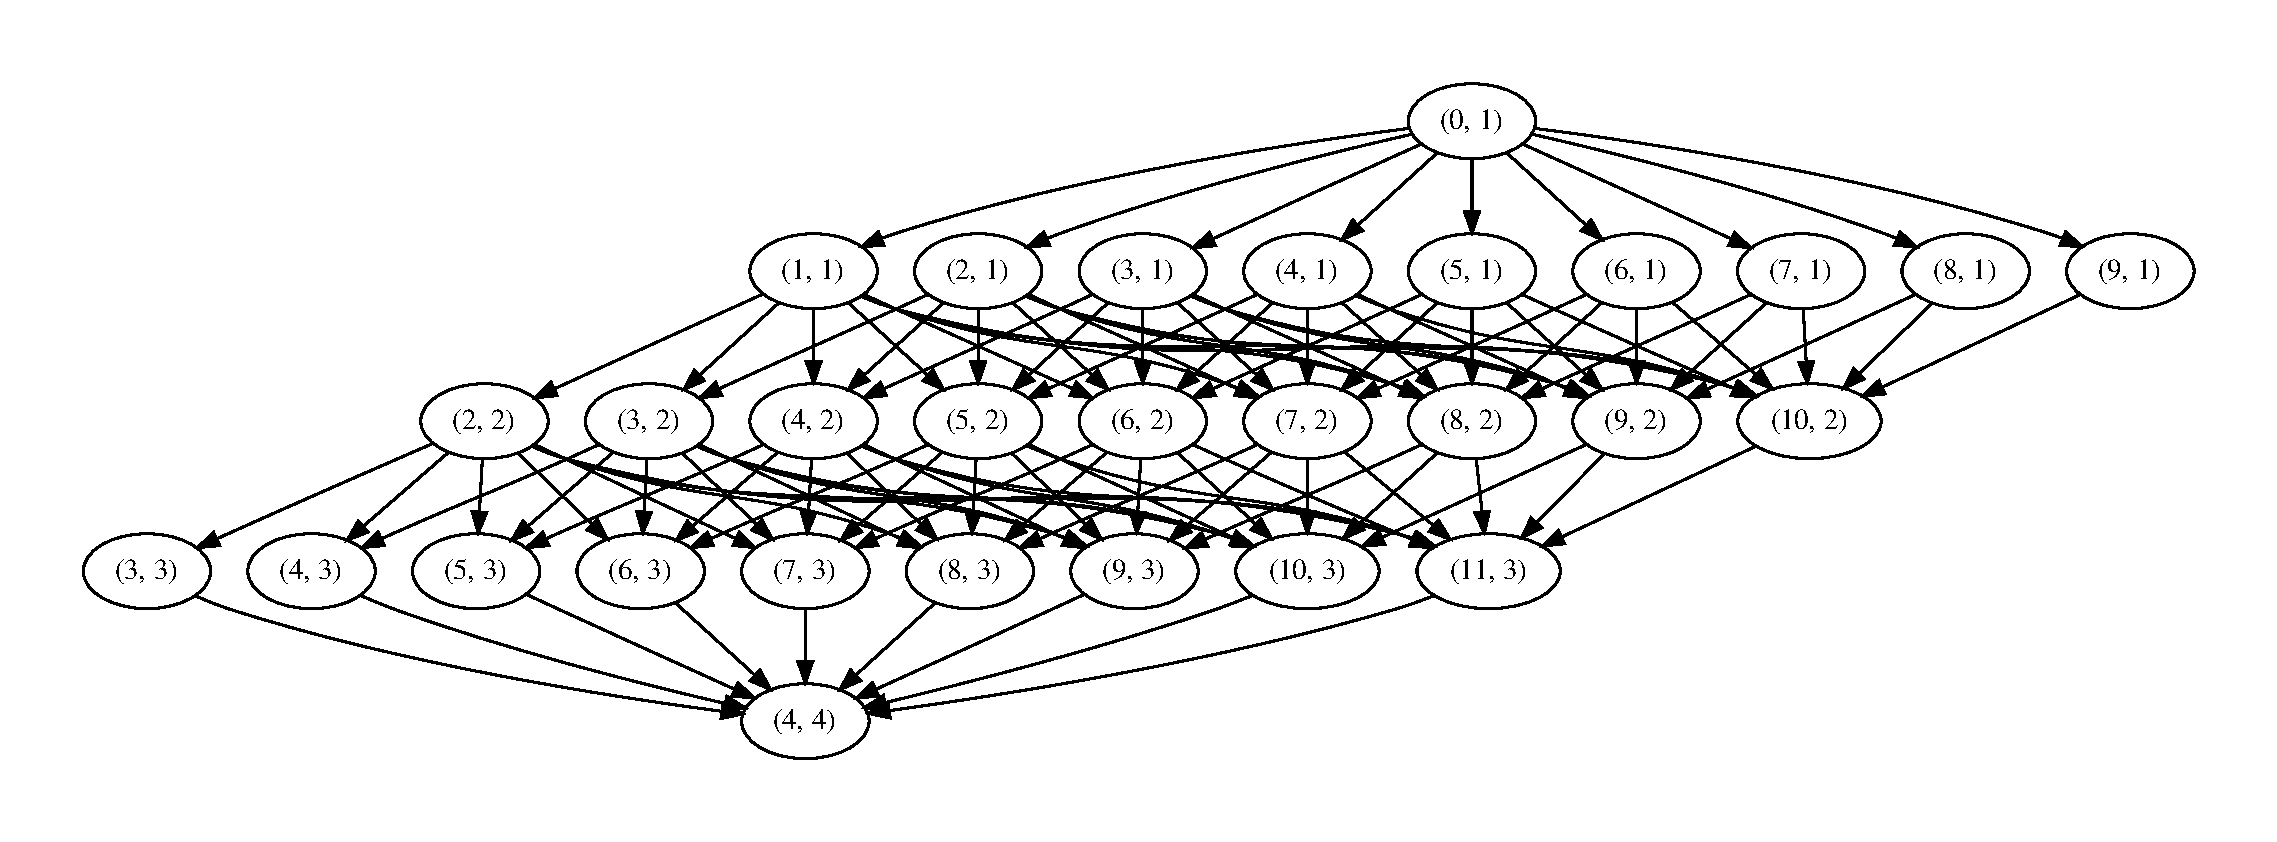
\includepdf[pages=-]{12_4_unlabeled.pdf}
% \begin{figure}
%   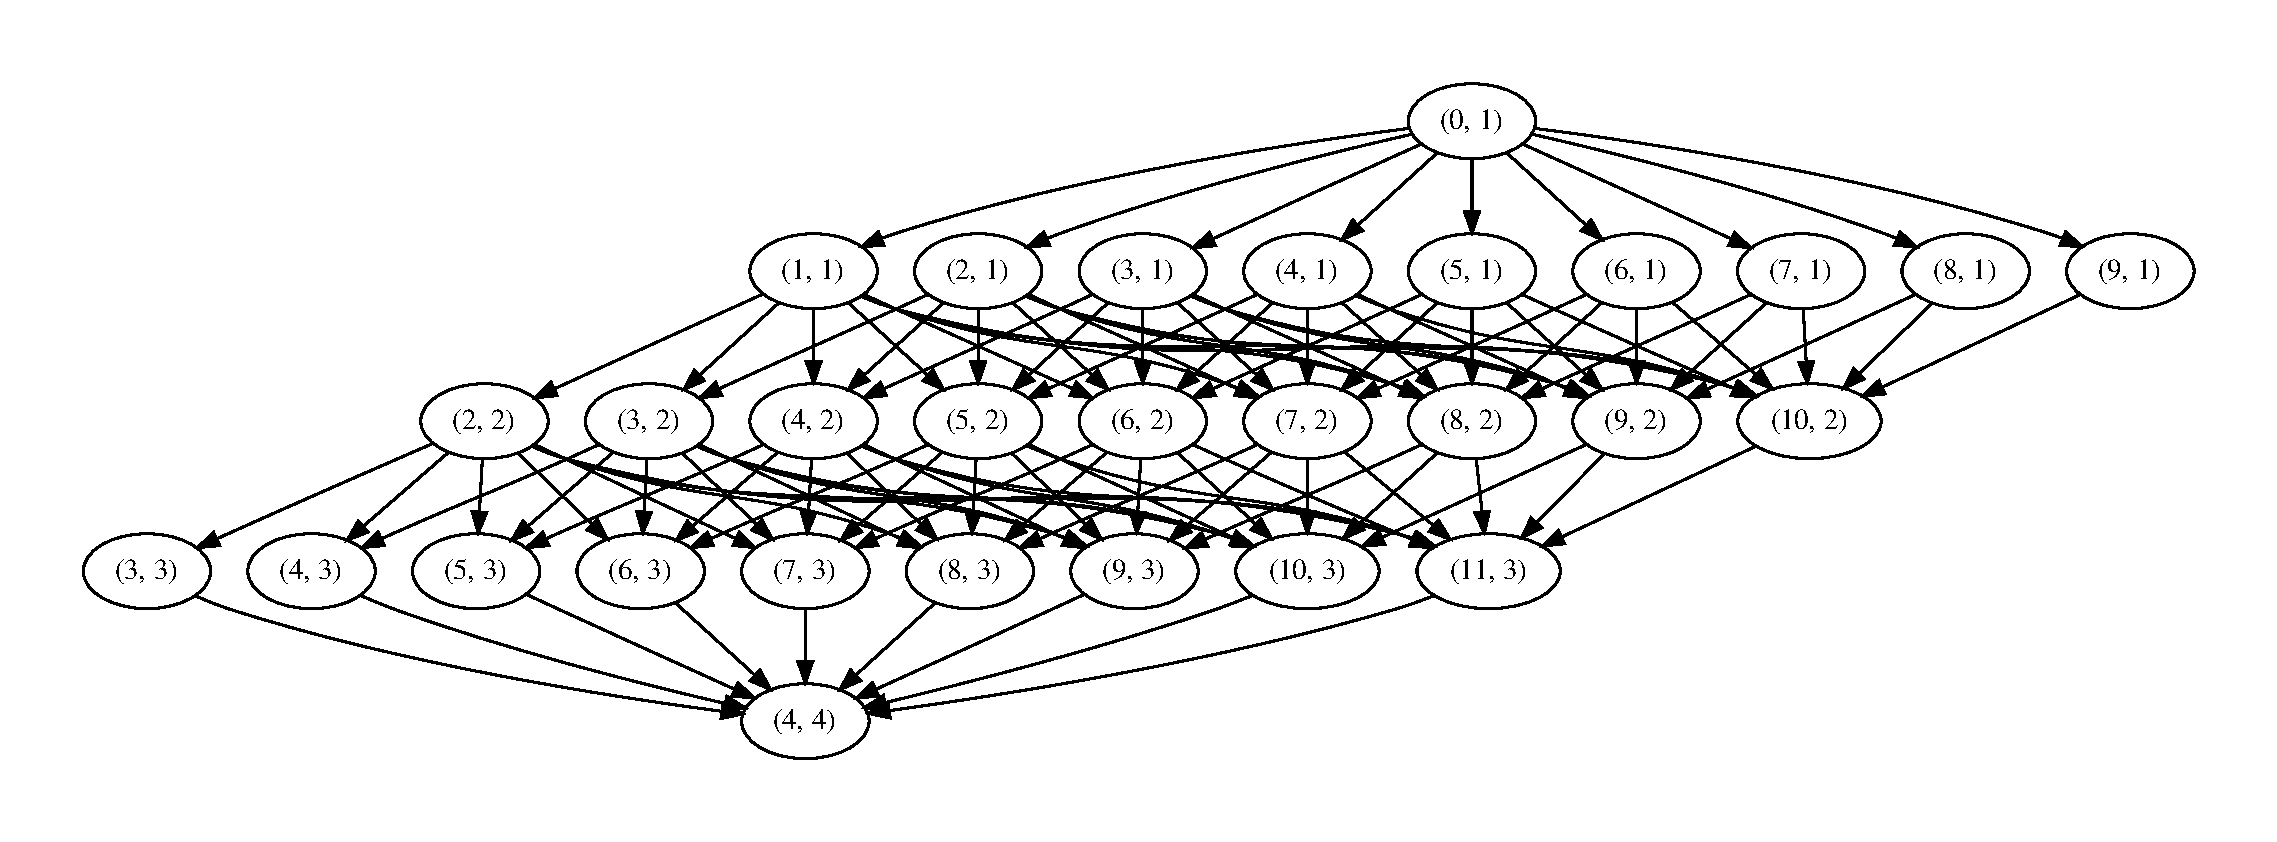
\includegraphics[scale=.22]{12_4_unlabeled.pdf}
%   \caption{Graph connectivity, (N, T) = (12, 4)}  
% \end{figure}

\vspace{16pt}
\begin{figure}
  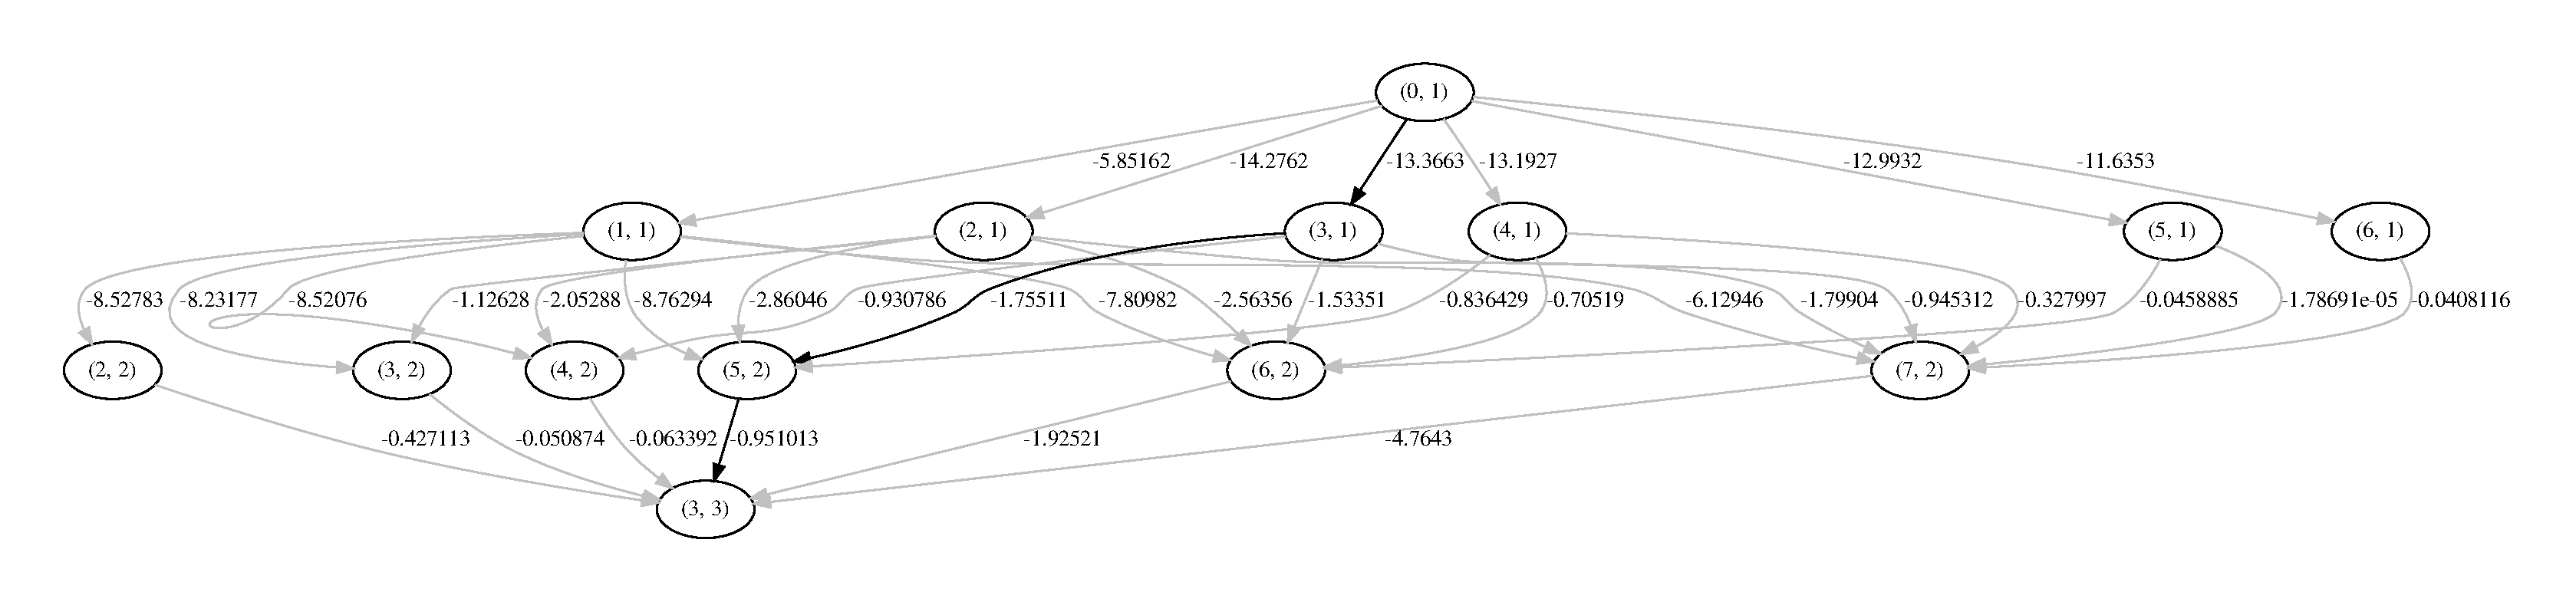
\includegraphics[scale=.25]{8_3_labeled.pdf}
  \caption{Labeled (N, T) = (8, 3) case displaying optimal path SOURCE -- (3, 1) -- (5, 2) --  SINK corresponding to ordered partition [[0 1 2 ], [3 4], [5 6 7 ]]}
\end{figure}

For the graph $\mathcal{G} = \left( V, E\right)$, we have 
\begin{align*}
\vert V \vert & = \left( T-1\right)\left(N-T-1\right) + 2 \\
\vert E \vert & = 2\left( N-T+1\right) + \left( T-1\right)\sum_{i=1}^{N-T+1} i = 2\left( N-T+1\right) + \frac{T-1}{2}\left( N-T+1\right)\left( N-T+2\right)
\end{align*}

The Bellman-Ford algorithm requires $\mathcal{O}\left( V\cdot E\right)$ operations, which for $N >> T$ is $\mathcal{O}\left( TN^2\right)$. A naive search of all ordered partitions requires $\binom{n-1}{T-1}$ operations, a polynomial of order $T-1$ in $N$. We have effectively reduced large cases to be no worse than quadratic in N. The time savings is at the expense of memory footprint; all partial sums of the form $\frac{-\left(\sum_{r=i}^{j-1} x_r\right)^2}{\sum_{r=i}^{j-1} y_r}$ must be stored (although sequential calculation cost is still $\mathcal{O}\left( N\right)$). This may be the most significant feature of this approach - all partial sums are cached on a computation tree that is easily traversed. For example, for a sample size of 10,000 points, with T = 100, there are approximately 4.8530e9 edges, with a storage cost of approximately 19.4119 Gb. Running times are quite fast, however, and we are currently exploring a distributed version of the algorithm.

\cleardoublepage
\appendix
\section{Appendix}
We present here an alternative proof of Theorem 1 which is more in the spirit of $\cite{article6}$, describing and exchange mechanism to swap elements between nonconsecutive subsets that terminates with all subsets consecutive.

\vspace{6pt}

$\textit{Proof of Theorem 1}$
For sufficiency, let $\gamma = 2$, and suppose the partition $\mathcal{P} = \left\lbrace P_1, \dots, P_T\right\rbrace$ is the argmax solution to \ref{eq1}. Let $R_1 = (X_1, Y_1)$ be the set of records in $\mathcal{P}$ that contains the maximal element $R_{(1)}$ of $\mathcal{D}$, and define $R_1^{in} = \argmin_{R_j \in X_1} G(x_i, y_i)$, $R_1^{out} = \argmax_{R_j \not\in X_1} G(x_i, y_i)$. Note that $X_1$ is an ordered subset if and only if $R_1^{in} <= R_1^{out}$, so that there are no "holes" in $X_1$. This is not true if $X_1$ does not contain the maximal element. This can be made precise by defining $I_1^{in} = j \text{ such that} R_{(j)} = R_1^{in}$, $I_1^{out} = j \text{ such that} R_{(j)} = R_1^{out}$, and $D_1 = I_1^{in} - I_1^{out}$. It is then the case that $D_1 \geq 1$, and $X_1$ is ordered if and only iff $D_1 < 0$.

Set $D = D_1$ and assume $D_1 \geq 0$. We describe an iterative procedure that swaps elements between $X_1$ and the remaining subsets, such that each step does not decrease the overall score of the partition, and decreases the value of $D$ by at least 1. In this way the procedure can be stopped when $X_1$ is ordered. We can then remove $X_1$ from the partition, regarding the remaining subsets as a partition of $\left\lbrace 1, \dots N-\vert X_1 \vert\right\rbrace$, and apply the same procedure to the remaining subset containing the maximal element. The process terminates with a maximal ordered partition.

\begin{algorithm}
\caption{Ordering Algorithm: Single Subset}
\begin{algorithmic}[1]
\State $\textit{Select } X_1 \textit{ containing maximal element of } \mathcal{D}$
\State $\left( \alpha , \beta \right) \gets R_1^{in}, \left( a,b \right) \gets R_1^{out}$
\State $D \gets I_1^{in} - I_1^{out}$
\While{$D \geq 0$}
\If{$X_1, X_2 \geq 0$}
\State $X_1^\prime \gets X_1\setminus \left\lbrace x_1^{in}\right\rbrace$, $Y_1^{\prime} \gets X_1\setminus \left\lbrace y_1^{in}\right\rbrace$
\State $X_2^{\prime} \gets X_2\cup \left\lbrace x_1^{in}\right\rbrace$, $Y_2^{\prime} \gets X_2\cup \left\lbrace y_1^{in}\right\rbrace$
\EndIf
\If{$X_1, X_2 \leq 0$}
\State $X_1^{\prime\prime} \gets X_1\cup \left\lbrace x_1^{out}\right\rbrace$, $Y_1^{\prime\prime} \gets X_1\cup \left\lbrace y_1^{out}\right\rbrace$
\State $X_2^{\prime\prime} \gets X_2\setminus \left\lbrace x_1^{out}\right\rbrace$, $Y_2^{\prime\prime} \gets X_2\setminus \left\lbrace y_1^{out}\right\rbrace$
\EndIf
\If{$X_1 \leq 0, X_2 \geq 0 \textit{ or } r X_1 \geq 0, X_2 \leq 0$}
\State $\left\lbrace X_1, Y_1, X_2, Y_2 \right\rbrace \gets \textit{one of } \left\lbrace X_1^{\prime}, Y_1^{\prime}, X_2^{\prime}, Y_2^{\prime}\right\rbrace, \left\lbrace X_1^{\prime\prime}, Y_1^{\prime\prime}, X_2^{\prime\prime}, Y_2^{\prime\prime}\right(\rbrace$
\EndIf
\State {$D \gets I_1^{in} - I_1^{out}$}
\EndWhile
\end{algorithmic}
\end{algorithm}

Without loss of generality, assume $R_1^{out} \in X_2$. We will assume that $G(x_1^{in}, y_1^{in}) < G(x_1^{out}, y_1^{out})$, and show that we can obtain an improvement in the sum $F(X_1, Y_1) + F(X_2, Y_2)$ by exchanging elements of $X_1$, $X_2$. In this way the elements of the subset $X_1$ are sucessively swapped out until it is ordered. Since $X_1$ is the partition with maximal element, we can remove it from consideration, and find the maximal remaining element, and apply the same procedure. In this way we obtain a partition all of whose subsets are ordered.

Assume the tuples $R_1^{in}$, $R_1^{out}$ are composed of $R_1^{in} = \left(x_1^{in}, y_1^{in}\right), R_1^{out} = \left(x_1^{out}, y_1^{out}\right)$.

Define
\begin{align*}
X^\prime\left( \lambda \right) & = \lambda \left( X_1 - x_1^{in}\right) + \left( 1 - \lambda\right) \left( X_1^\prime + x_1^{out}\right) \\
Y^\prime\left( \lambda \right) & = \lambda \left( Y_1 - y_1^{in}\right) + \left( 1 - \lambda\right) \left( Y_1^\prime + y_1^{out}\right)
\end{align*}

for $\lambda \in \left[ 0,1\right]$. For $\lambda_{*} = \frac{y_1^{out}}{y_1^{in} + y_1^{out}}$, we have $Y^\prime\left( \lambda_{*}\right) = Y_1$, and 
\[X^\prime\left( \lambda_{*}\right) = X_1 + \frac{y_1^{in}x_1^{out}-y_1^{out}x_1^{in}}{y_1^{in} + y_1^{out}}\]

Since $G(x_1^{in}, y_1^{in}) < G(x_1^{out}, y_1^{out})$, $\frac{y_1^{in}x_1^{out}-y_1^{out}x_1^{in}}{y_1^{in} + y_1^{out}} > 0$ and $X^\prime\left( \lambda_{*}\right) > 0$. We therefore have 
\begin{align} \label{eq2}
F(X_1, Y_1) \leq F(X^\prime\left( \lambda \right), Y_1) \leq \lambda\left( F(X_1-x_1^{in},Y_1-y_1^{in})\right) + \left( 1 + \lambda\right)\left( F(X_1+x_1^{out},Y_1+y_1^{out})\right)
\end{align}
where the second inequality is from the quasiconvexity of $F$ for $\gamma = 2$. From \ref{eq2} it follows that 
\begin{align} \label{eq3}
F(X_1, Y_1) \leq \max{\left(F(X_1-x_1^{in},Y_1-y_1^{in}), F(X_1+x_1^{out},Y_1+y_1^{out})\right)}
\end{align}

To get a similar result for the sets $X_2$, $Y_2$, define the transformed sequences $\bar{X} = \left\lbrace -x_1, \dots, -x_n\right\rbrace$, $\bar{Y} = \left\lbrace y_1, \dots, y_n\right\rbrace$. The sets $\bar{X_1}, \bar{X_2}, \bar{Y_1}, \bar{Y_2}$ are similarly defined, and we can define $\bar{R_2}^{in} = \argmin_{\bar{R_j} \in \bar{X_2}} G(\bar{x_i}, \bar{y_i})$, $\bar{R_1}^{out} = \argmax_{\bar{R_j} \not\in \bar{X_1}} G(\bar{x_i}, \bar{y_i})$. Assuming the correspondence between record and underlying sequences $\bar{R}_i = \left(\bar{x_i}, \bar{y_i}\right)$, we then have $x_1^{in} = -\bar{x}_2^{out}$, $y_1^{in} = \bar{y_2}^{out}$, and $x_1^{out} = -\bar{x}_2^{in}$, $y_1^{out} = \bar{y_2}^{in}$. 

Define
\begin{align*}
\bar{X}^\prime\left( \lambda \right) & = \lambda \left( \bar{X_2} - \bar{x_2}^{in}\right) + \left( 1 - \lambda\right) \left( \bar{X_2} + \bar{x_2}^{out}\right) \\
\bar{Y}^\prime\left( \lambda \right) & = \lambda \left( \bar{Y_2} - \bar{y_2}^{in}\right) + \left( 1 - \lambda\right) \left( \bar{Y_2} + \bar{y_2}^{out}\right)
\end{align*}

for $\lambda \in \left[ 0,1\right]$. For $\bar{\lambda}_{*} = \frac{\bar{y_2}^{out}}{\bar{y_2}^{in} + \bar{y_2}^{out}}$, we have $\bar{Y}^\prime\left( \bar{\lambda}_{*}\right) = \bar{Y_1}$, and 
\[\bar{X}^\prime\left( \bar{\lambda}_{*}\right) = \bar{X_2} + \frac{\bar{y_2}^{in}\bar{x_2}^{out}-\bar{y_2}^{out}\bar{x_2}^{in}}{\bar{y_2}^{in} + \bar{y_2}^{out}}\]
By similar arguments, and since $\bar{y_2}^{in}\bar{x_2}^{out}-\bar{y_2}^{out}\bar{x_2}^{in} = x_1^{out}y_1^{in} - x_1^{in}y_1^{out} \geq 0$, 
\begin{align*}
F(X_2, Y_2) = F(\bar{X_2}, \bar{Y_2}) & \leq \max{\left(F(\bar{X_2}-\bar{x_2}^{in},\bar{Y_2}-\bar{y_2}^{in}), F(\bar{X_2}+\bar{x_2}^{out},\bar{Y_2}+\bar{y_2}^{out})\right)} \\
& = \max{\left(F(\bar{X_2}-\bar{x_2}^{in},Y_2-y_1^{our}), F(\bar{X_2}+\bar{x_2}^{out},\bar{Y_2}+y_2^{out})\right)} \\
& = \max{\left(F(\bar{X_2} +x_1^{out},Y_2-y_1^{out}), F(\bar{X_2}-x_1^{in},Y_2+y_2^{out})\right)} \\
& = \max{\left(F(X_2 -x_1^{out},Y_2-y_1^{out}), F(X_2+x_1^{in},Y_2+y_2^{out})\right)}
\end{align*}

So
\begin{align} \label{eq4}
F(X_2, Y_2) \leq \max{\left(F(X_2-x_1^{out},Y_2-y_1^{out}), F(X_2+x_1^{in},Y_2+y_1^{in})\right)}
\end{align}

If we form the table
\[
\begin{pmatrix}
&F(X_1 - x_1^{in}, Y_1 - y_1^{in}) & F(X_2 + x_1^{in}, Y_2 + y_1^{in}) \\
&F(X_1 + x_1^{out}, Y_1 + y_1^{out}) & F(X_2 - x_1^{out}, Y_2 - y_1^{out})
\end{pmatrix} = \begin{pmatrix}
&A_{11} & A_{12} \\
&A_{21} & A_{22}
\end{pmatrix}
\]
then the results in \ref{eq2}, \ref{eq4} imply that $F(X_1, Y_1) \leq \max{\left(A_{11}, A_{21}\right)}$ and $F(X_2, Y_2) \leq \max{\left(A_{12}, A_{22}\right)}$. What we would like to show is that $F(X_1, Y_1) + F(X_2, Y_2) \leq \max{\left(A_{11}, A_{12}\right)}$ or $F(X_1, Y_1) + F(X_2, Y_2) \leq \max{\left(A_{21}, A_{22}\right)}$, as those operations represent a swap of records between the two sets $X_1$, $X_2$. To this end assume that the maximum values down columns occur in different rows, e.g. $\max{\left(A_{11}, A_{21}\right)} = A_{11}$, $\max{\left(A_{12}, A_{22}\right)} = A_{22}$. The case for which the maximums occur on the opposite diagonal is handled similarly. We can then assume that 
\begin{align}
& F(X_1 - x_1^{in}, Y_1 - y_1^{in}) - F(X_1, Y_1) \geq 0 \\
& F(X_2 - x_1^{out}, Y_2 - y_1^{out}) - F(X_2, Y_2) \geq 0 \\
& F(X_1 + x_1^{out}, Y_1 + y_1^{out}) - F(X_1, Y_1) \leq 0 \\
& F(X_2 + x_1^{in}, Y_2 + y_1^{in}) - F(X_2, Y_2) \leq 0
\end{align}

Expand 
\[
F(X - \alpha, Y - \beta) - F(X, Y) = \frac{\beta X^2 - 2\alpha XY + \alpha^2 Y}{Y\left( Y-\beta\right)}
\]
and write
\begin{align*}
F(X_1 - x_1^{in}, Y_1 - y_1^{in}) + F(X_2 + x_1^{in}, Y_2 + y_1^{in}) - \left( F(X_1, Y_1) + F(X_2, Y_2)\right) = \\
\left( F(X_1 - x_1^{in}, Y_1 - y_1^{in}) - F(X_1 - x_1^{in}, Y_1)\right) + \left( F(X_1 - x_1^{in}, Y_1) - F(X_1 , Y_1)\right) + \\
\left( F(X_2 + x_1^{in}, Y_2 + y_1^{in}) - F(X_2 + x_1^{in}, Y_2)\right) + \left( F(X_2 + x_1^{in}, Y_2) - F(X_2, Y_2)\right)
\end{align*}

and
\begin{align*}
F(X_1 + x_1^{out}, Y_1 + y_1^{out}) + F(X_2 - x_1^{out}, Y_2 - y_1^{out}) - \left( F(X_1, Y_1) + F(X_2, Y_2)\right) = \\
\left( F(X_1 + x_1^{out}, Y_1 + y_1^{out}) - F(X_1 + x_1^{out}, Y_1)\right) + \left( F(X_1 + x_1^{out}, Y_1) - F(X_1 , Y_1)\right) + \\
\left( F(X_2 - x_1^{out}, Y_2 - y_1^{out}) - F(X_2 - x_1^{out}, Y_2)\right) + \left( F(X_2 - x_1^{out}, Y_2) - F(X_2, Y_2)\right)
\end{align*}

For ease of notation designate $\alpha = x_1^{in}$, $\beta = y_1^{in}$, $a = x_1^{out}$, $b = y_1^{out}$.

The summands for the top equation can then be written
\begin{align*}
s_1 & = \frac{\left(X_1 - \alpha\right)^2\beta}{Y_1\left( Y_1 - \beta\right)} \\
s_2 & = \frac{\alpha \left( \alpha - 2X_1\right)}{Y_1} \\
s_3 & = \frac{-\left( X_2 + \alpha\right)^2\beta}{Y_2\left( Y_2 + \beta\right)} \\
s_4 & = \frac{\alpha\left( \alpha + 2X_2\right)}{Y_2}
\end{align*}

and the bottom
\begin{align*}
t_1 & = \frac{-\left( X_1 + a\right)^2 b}{Y_1\left( Y_1 + b\right)} \\
t_2 & = \frac{a\left( a + 2X_1\right)}{Y_1} \\
t_3 & = \frac{\left( X_2 - a\right)^2b}{Y_2\left( Y_2 - b\right)} \\
t_4 & = \frac{a\left( a - 2X_2\right)}{Y_2}
\end{align*}

We will show that the that one of
\begin{align} \label{eq5}
F(X_1 - \alpha, Y_1 - \beta) + F(X_2 + \alpha, Y_2 + \beta) - F(X_1, Y_1) - F(X_2, Y_2) & \geq 0 \\
F(X_1 + a, Y_2 +b) + F(X_2 - a, Y_2 - b) - F(X_1, Y_1) - F(X_2, Y_2) & \geq 0
\end{align}
holds.


\begin{case} 
$X_1 >= 0$, $X_2 >= 0$. 
\end{case}
We will show that the top row in \ref{eq5} is positive.

\vspace{12pt}

\begin{claim}
$\frac{X_1}{Y_1} \geq \frac{X_2}{Y_2}$, $\frac{X_1}{Y_1} \geq \frac{2a}{b}$, $\frac{X_2}{Y_2} \geq \frac{2\alpha }{\beta}$.
\end{claim}
\begin{claimproof}
Since $F(X - \alpha, Y - \beta) - F(X, Y) = \frac{\beta X^2 - 2\alpha XY + \alpha^2 Y}{Y\left( Y-\beta\right)}$ is a polynomial in $X$, we have
\begin{align*}
F(X_1+a, Y_1+b) - F(X_1,Y_1) \leq 0 & \implies X_1 \not \in \left( \frac{a}{b}Y_1 \pm \vert \frac{a}{b} \vert \sqrt{Y_1\left( Y_1+b\right) } \right) \\
& \implies \frac{X_1}{Y_1} \not \in \left( \frac{a}{b} \left( 1 \pm \frac{\sqrt{Y_1\left( Y_1+b\right) }}{Y_1}\right) \right)
\end{align*}
Since $\frac{X_1}{Y_1} \geq 0$, it follows that $\frac{X_1}{Y_1} \geq \frac{2a}{b}$. By similar reasoning, 
\begin{align*}
F(X_2+\alpha, Y_2+\beta) - F(X_2,Y_2) \leq 0 & \implies X_2 \not \in \left( \frac{\alpha}{\beta}Y_2 \pm \vert \frac{\alpha}{\beta} \vert \sqrt{Y_2\left( Y_2+\beta \right) } \right) \\
& \implies \frac{X_2}{Y_2} \not \in \left( \frac{\alpha}{\beta} \left( 1 \pm \frac{\sqrt{Y_2\left( Y_2+\beta \right) }}{Y_2}\right) \right)
\end{align*}
so that $\frac{X_2}{Y_2} \geq \frac{2\alpha}{\beta}$. Now since $\frac{2\alpha}{\beta} \leq \frac{X_1}{Y_2}$ and $\frac{\alpha}{\beta} \leq \frac{a}{b}$, it follows that $\frac{X_1}{Y_1} \geq \frac{X_2}{Y_2}$.
\end{claimproof}

\begin{claim}
$s_1 + s_3 \geq 0$
\end{claim}
\begin{claimproof}
\begin{align*}
s_1 = \frac{\left( X_1 - \alpha \right)^2\beta }{Y_1\left( Y_1 - \beta\right)} & = \frac{\beta}{Y_1-\beta}F(X_1+\alpha, Y_1) \\
s_3 = -\frac{\left( X_2 + \alpha \right)^2 \beta }{Y_2\left( Y_2+\beta\right) } & = \frac{-\beta}{Y_2 + \beta}F(X_2+\alpha, Y_2)
\end{align*}
So
\begin{align*}
s_1 + s_3 & = \frac{\beta}{Y_1-\beta}F(X_1+\alpha, Y_1) - \frac{\beta}{Y_2 + \beta}F(X_2+\alpha, Y_2) \\
& = \frac{\beta}{Y_1 - \beta}\left( F(X_1, Y_1) + s_2\right) - \frac{\beta}{Y_2 + \beta}\left( F(X_2,Y_2) + s_4\right)
\end{align*}
Since $F(X - \alpha, Y - \beta) - F(X, Y) = \frac{\beta X^2 - 2\alpha XY + \alpha^2 Y}{Y\left( Y-\beta\right)}$, 
\begin{align*}
F(X_1 - \alpha, Y_1 - \beta) - F(X_1, Y_1) \geq 0 & \implies \beta \geq \frac{\alpha Y_1}{X_1^2}\left( 2X_1 - \alpha \right) \implies s_2 \geq -\frac{\beta}{Y_1}F(X_1, Y_1) \\
F(X_2+\alpha, Y_2+\beta) - F(X_2, Y_2) \leq 0 & \implies \beta \geq \frac{Y_2}{X_2^2}\left( 2X_2 + \alpha \right) \implies s_4 \leq \frac{\beta}{Y_2}F(X_2, Y_2)
\end{align*}
So 
\begin{align*}
s_1 + s_3 & \geq \frac{\beta}{Y_1 - \beta}\left( F(X_1, Y_1) - \frac{\beta}{Y_1}F(X_1, Y_1)\right) - \frac{\beta}{Y_2+\beta}\left( F(X_2, Y_2) + \frac{\beta}{Y_2}F(X_2, Y_2)\right) \\
& = \frac{\beta}{Y_1}F(X_1, Y_1) - \frac{\beta}{Y_2}F(X_2, Y_2) \\
& = \beta \left( \left( \frac{X_1}{Y_1}\right)^2 - \left( \frac{X_2}{Y_2}\right)^2 \right) \\
& \geq 0,
\end{align*}
by the previous claim, and that all quantities are positive.

\end{claimproof}
\begin{claim}
$\sum_{i=1}^{4} s_i \geq 0$
\end{claim}
\begin{claimproof}
\begin{align*}
s_2 + s_4 & = F(X_1 +\alpha, Y_1) - F(X_1, Y_1) + F(X_2 + \alpha, Y_2) - F(X_2, Y_2) \\
& = \frac{\alpha \left( \alpha - 2X_1\right)}{Y_1} + \frac{\alpha \left( \alpha + 2X_2\right)}{Y_2}
\end{align*}
As a polynomial in $\alpha$ we have
\[
s_2 + s_4 = p(\alpha) = \alpha \left( g + \frac{1}{2}h \alpha \right),
\]
where
\begin{align*}
g & = \frac{2 \left( X_2 Y_1 - X_1 Y_2\right)}{Y_1 Y_2} \\
h & = \frac{Y_1 + Y_2}{Y_1 Y_2}
\end{align*}
So $p$ has two real roots, one at $\alpha_1 = 0$ and one for $\alpha_2 \geq 0$. The graph is an upward parabola so that $p \geq 0$ for $\alpha \leq 0$, so the remaining case is $\alpha > 0$. We have, as above
\begin{align*}
F(X_1-\alpha, Y_1-\beta) - F(X_1, Y_1) \geq 0 & \implies \alpha \not \in \left( X_1 \pm \vert X_1\vert \sqrt{\frac{Y_1-\beta}{Y_1}}\right) \\
F(X_2+\alpha, Y_2+\beta) - F(X_2, Y_2) \leq 0 & \implies \alpha \not \in \left( -X_2 \pm \vert X_2\vert \sqrt{\frac{Y_2 +\beta}{Y_2}} \right)
\end{align*}
so that $\alpha > 0$ means that $\alpha \in \left[ 0, \min{X_1\left( 1 - \sqrt{\frac{Y_1-\beta}{Y_1}}\right), X_2\left( \sqrt{\frac{Y_2 + \beta}{Y_2} - 1} \right)}\right]$. The idea is that $\alpha$ is small relative to $\beta$ so that the polynomial $p(\alpha) = s_2 + s_4$ never goes negative enough to violate $s_1 + s_2 \leq -\left( s_1 + s_3\right)$. The proof is technical and is below.
\end{claimproof}

\begin{lemma}
For $X_1$, $X_2 > 0$, $alpha \geq 0$, $s1 + s3 \geq 0$, we have $\sum_i s_i \geq 0$
\end{lemma}
\begin{proof}
We can write
\begin{align*}
s_2 + s_4 & = \frac{\alpha \left( \alpha - 2X_1\right)}{Y_1}  + \frac{\alpha\left( \alpha + 2X_2\right)}{Y_2} \\
& = \left( \frac{Y_1}{Y_2} + \frac{Y_2}{Y_1}\right)\alpha^2 + 2\left( \frac{X_2}{Y_2} - \frac{X_1}{Y_1} \right)\alpha
\end{align*}
By the proof of the claim tha $s_1 + s_3 \geq 0$, we have that $s_1 + s_3 \geq \beta \left( \left( \frac{X_1}{Y_1}\right)^2 - \left( \frac{X_2}{Y_2}\right)^2 \right)$, so it is sufficient to show that
\[
\left( \frac{Y_1}{Y_2} + \frac{Y_2}{Y_1}\right)\alpha^2 + 2\left( \frac{X_2}{Y_2} - \frac{X_1}{Y_1} \right)\alpha \geq  - \beta\left( \left( \frac{X_1}{Y_1}\right)^2 - \left( \frac{X_2}{Y_2}\right)^2 \right)
\]
Writing the left-hand side as $q\left( \alpha \right) = h\alpha^2 + g\alpha + c$, it is sufficient to show that $\vert \alpha\vert \vert g + h \alpha\vert \leq \vert \beta\left( \left( \frac{X_1}{Y_1}\right)^2 - \left( \frac{X_2}{Y_2}\right)^2 \right) \vert$. By elementary methods, and the fact that 
\begin{align*}
F(X_1-\alpha, Y_1-\beta) - F(X_1, Y_1) \geq 0 & \implies \alpha \not \in \left( X_1 \pm \vert X_1\vert \sqrt{\frac{Y_1-\beta}{Y_1}}\right) \\
F(X_2+\alpha, Y_2+\beta) - F(X_2, Y_2) \leq 0 & \implies \alpha \not \in \left( -X_2 \pm \vert X_2\vert \sqrt{\frac{Y_2 +\beta}{Y_2}} \right)
\end{align*}
so that $\alpha > 0$ means that $\alpha \in \left[ 0, \min{X_1\left( 1 - \sqrt{\frac{Y_1-\beta}{Y_1}}\right)}\right]$, it can be shown that since $h \leq 0$, $g \geq 0$, $\vert \alpha\vert \vert g + h \alpha\vert \leq \vert \alpha g \vert$. Finally,
\begin{align*}
\vert \alpha g \vert = 2\alpha\left( \frac{X_1}{Y_1} - \frac{X_2}{Y_2}\right) & \leq \beta\left( \left(\frac{X_1}{Y_1}\right)^2 - \left(\frac{X_2}{Y_2}\right)^2\right) \\
\iff 2\alpha & \leq \beta\left( \frac{X_1}{Y_1} + \frac{X_2}{Y_2}\right)
\end{align*}
By the claim, we have $\frac{X_1}{Y_1} \geq \frac{\alpha}{\beta}$, $\frac{X_2}{Y_2} \geq \frac{2\alpha}{\beta}$, which proves the lemma.

\end{proof}

\begin{case}
$X_1$,  $X_2 \leq 0$
\end{case}
Writing the transformed sets $\bar{X_1} = -X_1$, $\bar{Y_1} = Y_1$, $\bar{X_2} = -X_2$, $\bar{Y_2} = Y_2$, and defining $\eta = \bar{x_2}^{in}$, $\theta = \bar{y_2}^{in}$, we have $a = -\eta$, $b = \theta$ by definition. Assume that $\bar{X_2}$ has the maximal element. We proceed as in case 1:
\begin{align*}
F(X_1, Y_1) + F(X_2, Y_2) = F(\bar{X_2}, \bar{Y_2}) + F(\bar{X_1}, \bar{Y_1}) & \leq F(\bar{X_2} - \eta, \bar{Y_2} - \theta) + F(\bar{X_1} + \eta, \bar{Y_1} + \theta) \\
& = F(-\left( \bar{X_2} - \eta\right), Y_2 - \theta) + F(-\left( \bar{X_1} + \eta \right), Y+2 + \theta) \\
& = F(X_2 + \eta, Y_2 - \theta) + F(X_1 - \eta, Y_2 + \theta) \\
& = F(X_2 - a, Y_2 - b) + F(X_1 + a, Y_1 + b)
\end{align*}
so that the bottom row represents an improvement to the original partition.
Note that if the maximal element lies in $\bar{X_1}$, then defining $\lambda = \bar{x_1}^{in}$, $\epsilon = \bar{y_1}^{in}$, we have $\lambda = x_{max}$, $\epsilon = y_{max}$, where $x_{max}$, $y_{max}$ are associated with the maximum priority record $R_{(1)}$ in $\mathcal{D}$. Then
\begin{align*}
F(X_1, Y_1) + F(X_2, Y_2) = F(\bar{X_2}, \bar{Y_2}) + F(\bar{X_1}, \bar{Y_1}) & \leq F(\bar{X_1} - \lambda, \bar{Y_1} - \epsilon) + F(\bar{X_2} + \lambda, \bar{Y_2} + \epsilon) \\
& = F(-\left( \bar{X_1} - \lambda\right), Y_1 - \epsilon) + F(-\left( \bar{X_2} + \lambda \right), Y_2 + \epsilon) \\
& = F(X_1 + \lambda, Y_1 - \epsilon) + F(X_2 - \lambda, Y_2 + \epsilon) \\
& = F(X_1 - x_{max}, Y_1 - y_{max}) + F(X_2 + x_{max}, Y_2 + y_{max})
\end{align*}
Now defining $X_1 = X_1\setminus\left\lbrace \right\rbrace$ If $X_1, X_2 \geq 0$, the previous argument applies, and 


After exchanging the maximal record between $X_1$, $X_2$, define the new partitions $X_1 = X_2\cup \left\lbrace x_{max}\right\rbrace$, $Y_1 = Y_2\cup \left\lbrace y_{max}\right\rbrace$, $X_2 = X_1\setminus \left\lbrace x_{max}\right\rbrace$, $Y_2 = Y_1\setminus \left\lbrace y_{max}\right\rbrace$, it follows that $X_1 \geq 0$. If $X_2 \geq 0$, the previous argument applies and $F(X_1, Y_1) + F(X_2, Y_2) \leq F(X_1 - x_{max}, Y_1 - y_{max}) + F(X_2 + x_{max}, Y_2 + y_{max})$. If $X_2 \leq 0$, we retain $X_1$ as the partition containing the maximal record, and since it no longer contains the miminal record, we must only make this change of designation once, and continue element exchange as in the remaining cases. Note that the swapping out of the maximal element only occurs once, then necessarily the new $X_1$ does not contain the minimal record.

\begin{case}
$X_1 \geq 0$, $X_2 \leq 0$
\end{case}
\begin{claim}
One of $s_1 + s_3$,  $t_1 + t_3$ is positive.
\end{claim}
\begin{claimproof}
From the claim above, 
\begin{align} \label{eq6}
s_1 + s_3 \geq \beta \left( \left( \frac{X_1}{Y_1}\right)^2 - \left( \frac{X_2}{Y_2}\right)^2 \right)
\end{align}
In this case we don't necessarily know that $F(X_1, Y_1) \geq F(X_2, Y_2)$. We have
\begin{align*}
t_1 = \frac{-\left( X_1 + a \right)^2b }{Y_1\left( Y_1 + b\right)} & = \frac{b}{Y_1+b}F(X_1+a, Y_1) \\
t_3 = -\frac{\left( X_2 - a \right)^2 b }{Y_2\left( Y_2-b\right) } & = \frac{b}{Y_2 -b}F(X_2-a, Y_2)
\end{align*}
So
\begin{align*}
t_1 + t_3 & = \frac{b}{Y_2-b}F(X_2 - a,Y_2) - \frac{-b}{Y_1 + b}F(X1 + a, Y_1) \\
& = \frac{b}{Y_2-b}\left( F(X_2, Y_2) + t_2\right) - \frac{-b}{Y_1 + b}\left( F(X_1, Y_1) + t_4\right)
\end{align*}
Since $F(X - \alpha, Y - \beta) - F(X, Y) = \frac{\beta X^2 - 2\alpha XY + \alpha^2 Y}{Y\left( Y-\beta\right)}$, 
\begin{align*}
F(X_2 - a, Y_2 - b) - F(X_2, Y_2) \geq 0 & \implies b \geq \frac{a Y_2}{X_2^2}\left( 2X_2 - a \right) \implies t_4 \geq \frac{-b}{Y_2}F(X_2, Y_2) \\
F(X_1+a, Y_1+b) - F(X_1, Y_1) \leq 0 & \implies b \geq \frac{aY_1}{X_1^2}\left( 2X_1 + a \right) \implies t_2 \leq \frac{b}{Y_1}F(X_1, Y_1)
\end{align*}
So 
\begin{align*}
t_1 + t_3 & \geq \frac{b}{Y_2 - b}\left( F(X_2, Y_2) - \frac{b}{Y_2}F(X_2, Y_2)\right) - \frac{b}{Y_1+b}\left( F(X_1, Y_1) + \frac{b}{Y_1}F(X_1, Y_1)\right) \\
& = \frac{b}{Y_2}F(X_2, Y_2) - \frac{b}{Y_1}F(X_1, Y_1) \\
& = b \left( \left( \frac{X_2}{Y_2}\right)^2 - \left( \frac{X_1}{Y_1}\right)^2 \right) \\
\end{align*}
This along with \ref{eq6} proves the claim.
\end{claimproof}

\begin{claim}
One of $\sum_{i=1}^4 s_i$ or $\sum_{i=1}^4 t_i$ is positive.
\end{claim}
\begin{claimproof}
Define $S =\sum_{i=1}^4 s_i$, $T = \sum_{i=1}^4 t_i$. We first examing the case $\alpha \leq 0$. By the claim above, one of $s_1 + s_3$, $t_1 + t_3$ is positive. Since
\[
s_2 + s_4 = \frac{\left( X_1 - \alpha\right)^2 - X_1^2}{Y_1} + \frac{\left( X_2 + \alpha\right)^2 - X_2^2}{Y_2} 
\]
it is clear that if $s_1 + s_3$ is positive, then $S$ is. So suppose $s_1 + s_3 \leq 0$ and $t_1 + t_3 \geq 0$. Then since
\[
t_2 + t_4  = \frac{\left( X_1 + a\right)^2 - X_1^2}{Y1} + \frac{\left( X_2 - a\right)^2 - X_2^2}{Y_2}
\]
we have $T \geq 0$ if $a \leq 0$. We have
\begin{align*}
F(X_1+a, Y_1+b) - F(X_1, Y_1) \leq 0 & \implies a \in \left[ -X_1 \pm \vert X_1\vert \sqrt{\frac{Y_1+b}{Y_1}}\right) \\
F(X_2-a, Y_2-b) - F(X_2, Y_2) \geq 0 & \implies a \not \in \left( X_2 \pm \vert X_2\vert \sqrt{\frac{Y_2 -b}{Y_2}} \right)
\end{align*}
so that $a > 0$ means that $a \in \left[ 0, \min{X_1\left( \sqrt{\frac{Y_1+b}{Y_1}} - 1\right), X_2\left( 1 - \sqrt{\frac{Y_2-b}{Y_2}} \right)}\right]$. Again we show that $t_2 + t_4$ is a polynomial in $a$, with real roots at $a = 0$ and $a > 0$, and that with this constraint on $a$, we never violate $t_2 + t_4 \leq -\left( t_1 + t_3\right)$. The proof is technical and is given in the appendix.
For $\alpha \geq 0$. note that this condition implies that all elements of $X_1$ are nonnegative. We can again replace $X_1$, $X_2$ with $\bar{X_1} = -X_1$, $\bar{X_2} = -X_2$, with $\bar{\alpha} = \argmin_{R_j \in \bar{X_2}} G(x_i, y_i) \leq 0$. The previous subcase for $\alpha \leq 0$ can then be invoked. Alternatively, we could argue along similar lines using $X_1$, $X_2$, noting that $\frac{\alpha}{\beta} \leq \frac{a}{b}$ implies that $a \geq 0$. Since $t_2 + t_4 \geq 0$ in this case, we have that $t_1 + t_3 \geq 0$ forces $T \geq 0$. If $s_1 + s_3 \geq 0$, then one of $S$, $T$ is positive as in the previous case.
\end{claimproof}

\begin{case}
$X_1 \leq 0$, $X_2 \geq 0$
\end{case}
Defining $\bar{X_1} = -X_1$, $\bar{Y_1} = Y_1$, and $\bar{X_2} = -X_2$, $\bar{Y_2} = Y_2$ will allow us to use the previous case, if the minimal element $\bar{R_{(n)}}$ lies in $\bar{X_1}$, so that the maximal element is in the positive partition in that case. This is true if and only if the minimal element of the original partition, $m = R_{(n)}$, does not lie in $X_2$. If it did, then direct computation of $F(X_1 + m, Y_1 + n) - F(X_1, Y_1)$, $F(X_2 - m, Y_2 + n) - F(X_2, Y_2)$ shows that the sum $F(X_1 + m, Y_1 + m) + F(X_2 - m, Y_2 - m)$ is positive, and represents an improvement to the original partition. So we can assume that $m \not \in X_2$, and the positive partition $\bar{X_1}$ contains the maximal element, and the previous case can be applied.

In this way the maximal subset $X_1$ is altered, without a decrease in the partition score, until $D_1 < 0$. $X_1$ is then ordered, and the partition $\mathcal{P} \setminus X_1$ of the set $\left\lbrace 1, \dots, N - \vert X_1\vert\right\rbrace$ is used in the next iteration.

\vspace{16pt}

The attention to subset membership of maximal and minimal records seems necessary. For the case $X1 \leq 0$, $X2 \leq 0$ (Case 2 above) for which the maximal element is in $X_1$ while the minimal element $m = R_{(n)}$ lies in $X_2$, we may not be able to effect an improvement in score by transferring any of the records $\left( x_1^{in}, y_1^{in}\right)$ or $\left( x_1^{out}, y_1^{out}\right)$. between the two subsets. For example, consider the case for $\left( N, T\right) = \left( 4, 2\right)$, with $X = [-5.64, -5.12, 10.0,  1.94]$, $Y = [0.077, 1.23 , 3.36, 0.029]$, and the suboptimal, unordred partition $\left[ \left[ 1, 2\right], \left[ 0, 3\right] \right] = \left[ X_2, X_1\right]$. The sequences are already sorted according to the standard priority. There are 6 partitions of $\left\lbrace 1, 2, 3, 4\right\rbrace$, and in this case $R_1^{in}$, $R_1^{out}$ correspond to the indices 0, 2, respectively. The normal substitutions considered in the proof are
\begin{align*}
\left[ X_2 + R_1^{in}, X_1 - R_1^{in}\right] & = \left[ \left[0,1,2] \right], \left[ 3\right] \right] \\
\left[ X_2 - R_1^{out}, X_1 + R_1^{out}\right] & = \left[ \left[ 1 \right], \left[ 0, 2, 3 \right] \right]
\end{align*}

In this case neither of the two partitions represent an improvement. The optimal partition is $\left\lbrace \left[ 0 \right], \left[ 1, 2, 3\right]\right\rbrace$ and represents the only improvement over the original partition:

\begin{verbatim}
SEQUENCES:
x = array([-5.64, -5.12, 10.0,  1.94])
y = array([0.077, 1.23 , 3.36, 0.029])
x/y = array([-73.24675325,  -4.16260163,   2.97619048,  66.89655172])

INDEX: 0 PARTITION: [[0, 1, 2], [3]]
    SUBSET: [0, 1, 2] SCORE: 0.12376258838654375
    SUBSET: [3] 		 SCORE: 129.77931034482756
    FINAL SCORE: 129.9030729332141
INDEX: 1 PARTITION: [[0, 2], [1, 3]]
    SUBSET: [0, 2]    SCORE: 5.530869944719233
    SUBSET: [1, 3]    SCORE: 8.032088959491661
    FINAL SCORE: 13.562958904210895
INDEX: 2 PARTITION: [[0], [1, 2, 3]]
	SUBSET: [0]       SCORE: 413.1116883116883
    SUBSET: [1, 2, 3] SCORE: 10.069798657718122
    FINAL SCORE: 423.1814869694064
INDEX: 3 PARTITION: [[0, 1], [2, 3]]
    SUBSET: [0, 1]    SCORE: 88.58270849273144
    SUBSET: [2, 3]    SCORE: 42.06656830923576
    FINAL SCORE: 130.6492768019672
INDEX: 4 PARTITION: [[0, 1, 3], [2]]
    SUBSET: [0, 1, 3] SCORE: 58.227844311377254
    SUBSET: [2]       SCORE: 29.761904761904763
    FINAL SCORE: 87.98974907328201
INDEX: 5 PARTITION: [[0, 3], [1, 2]]
    SUBSET: [0, 3]    SCORE: 129.1509433962264
    SUBSET: [1, 2]    SCORE: 5.188322440087146
    FINAL SCORE: 134.33926583631356
INDEX: 6 PARTITION: [[0, 2, 3], [1]]
    SUBSET: [0, 2, 3] SCORE: 11.451240623196773
    SUBSET: [1]       SCORE: 21.312520325203252
    FINAL SCORE: 32.76376094840003
MAX_SUM: 423.1814869694064, MAX_PARTITION: [[0], [1, 2, 3]]

\end{verbatim}



It is not clear how to achieve the optimal partition in one step. Even the substitution
\[
\left[ X_2 + R_1^{in} - R_1^{out}, X_1 - R_1^{in}+R_1^{out} \right] = \left[ \left[0,1] \right], \left[ 2, 3\right] \right]
\]
does not represent an improvemnt. The improvement is obtained by substition to obtain $\left[ \left[ 0 \right], \left[ 1, 2, 3\right]\right]$, from the original $\left[ \left[ 1, 2\right], \left[ 0, 3\right] \right]$, by moving the maximal item from $X_1$ to $X_2$, and doesn't touch $R_1^{in}$ nor $R_1^{out}$.

In this case it is seems necessary to remove the maximal element from $X_1$ to get to $\left[ \left[ 0 \right], \left[ 1, 2, 3\right]\right]$, which is the operation perfomed in that case above. The partition is then ordered, so the algorithm halts, but if it weren't, we would have $X_1 \leq 0$, $X_2 \geq 0$, the maximal record now in $X_2$, which would become the new $X_1$, and the algorithm would proceed. 


\begin{thebibliography}{1}

   \bibitem{article1} Chakravarty, A. K., J. B. Orlin, and U. G. Rothblum. A partitioning problem with additive objective with an application to optimal inventory groupings for joint replenishment. {\em Operations Research}. 30, no. 5, 1982: 1018-1022.

    \bibitem{article2} Chakravarty, Amiya K., James B. Orlin, and Uriel G. Rothblum. Consecutive optimizers for a partitioning problem with applications to optimal inventory groupings for joint replenishment. {\em Operations Research}. 33, no. 4, 1985: 820-834

	\bibitem{article 2} M. Kulldorff. A spatial scan statistic. {\em Communications in Statistics: Theory and Methods}, 26(6), 1997: 1481–1496

	\bibitem{article3} M. Kulldorff and N. Nagarwalla. Spatial disease clusters: detection and inference. {\em Statistics in Medicine}, 14, 1995: 799–810
	
	\bibitem{article4} Graham, R.L. (1972). "An Efficient Algorithm for Determining the Convex Hull of a Finite Planar Set" (PDF). Information Processing Letters. 1 (4): 132–133. doi:10.1016/0020-0190(72)90045-2.	
	
	\bibitem{article5} Eric V. Denardo, Gur Huberman and Uriel G. Rothblum. Optimal Locations on a Line Are Interleaved. {\em Operations Research}, Vol. 30, No. 4 (Jul. - Aug., 1982), pp. 745-759

	\bibitem{article6} Daniel B. Neill, Fast subset scan for spatial pattern detection. {\em Journal. Royal Statist. Soc.} B (2012) 74, Part 2, pp. 337–360
	
	\bibitem{article7} Learning with Submodular Functions: A Convex Optimization Perspective, Francis Bach Carnegie Mellon University, Pittsburgh, USA

\end{thebibliography}

\end{document}
